% Pengaturan ukuran teks dan bentuk halaman dua sisi
\documentclass[12pt]{report}

% Pengaturan ukuran halaman dan margin
\usepackage[a4paper,top=30mm,left=30mm,right=20mm,bottom=25mm]{geometry}

% Pengaturan ukuran spasi
\usepackage[singlespacing]{setspace}

% Judul dokumen
\title{Proposal Tugas Akhir ITS}
\author{Solang, Dion Andreas}

% Pengaturan detail pada file PDF
\usepackage[pdfauthor={\@author},bookmarksnumbered,pdfborder={0 0 0}]{hyperref}


% Pengaturan ukuran indentasi
\setlength{\parindent}{2em}

% Package lainnya
\usepackage{changepage}
\usepackage{etoolbox} % Mengubah fungsi default

% Pengaturan jenis karakter
\usepackage[utf8]{inputenc}

\usepackage[style=apa, 
  backend=biber,
  citestyle=authoryear-comp]{biblatex}
\usepackage{enumitem} % Pembuatan list
\usepackage{lipsum} % Pembuatan template kalimat
\usepackage{graphicx} % Input gambar
\usepackage{longtable} % Pembuatan tabel
\usepackage[table,xcdraw]{xcolor} % Pewarnaan tabel
\usepackage{eso-pic} % Untuk menggunakan background image di halaman
\usepackage{txfonts} % Font times
\usepackage{changepage} % Pembuatan teks kolom
\usepackage{multicol} % Pembuatan kolom ganda
\usepackage{multirow} % Pembuatan baris ganda
\usepackage{tabularx} % Untuk mengatur kolom, seperti grid pada CSS
\usepackage{wrapfig}

% Definisi untuk "Hati ini sengaja dikosongkan"
\patchcmd{\cleardoublepage}{\hbox{}}{
  \thispagestyle{empty}
  \vspace*{\fill}
  \begin{center}\textit{[Halaman ini sengaja dikosongkan]}\end{center}
  \vfill}{}{}

  % Pengaturan penomoran halaman
\usepackage{fancyhdr}
\fancyhf{}
\renewcommand{\headrulewidth}{0pt}
\pagestyle{fancy}
\fancyfoot[C,CO]{\thepage}
\patchcmd{\chapter}{plain}{fancy}{}{}
\patchcmd{\chapter}{empty}{plain}{}{}

% Pengaturan format judul bab
\usepackage{titlesec}
\renewcommand{\thesection}{\thechapter.\arabic{section}}
\titleformat{\chapter}[hang]{\centering\bfseries\Large}{BAB\ \arabic{chapter}\ }{0ex}{\vspace{0ex}\centering}
\titleformat*{\section}{\large\bfseries}
\titleformat*{\subsection}{\normalsize\bfseries}
\titlespacing{\chapter}{0ex}{6ex}{3ex}
\titlespacing{\section}{0ex}{3ex}{1.5ex}
\titlespacing{\subsection}{0ex}{3ex}{1.5ex}
\titlespacing{\subsubsection}{0ex}{0.5ex}{0ex}
\setcounter{secnumdepth}{3} % Untuk memberi penomoran pada \subsubsection

% Pengaturan daftar isi

\usepackage{tocloft}
\setlength{\cftsecindent}{2em}
\setlength{\cftsubsecindent}{2em}
\setlength{\cftbeforechapskip}{1.5ex}
\setlength{\cftbeforesecskip}{1.5ex}
\setlength{\cftbeforetoctitleskip}{0cm}
\setlength{\cftbeforeloftitleskip}{0cm}
\setlength{\cftbeforelottitleskip}{0cm}
\renewcommand{\cftsecfont}{\normalfont\bfseries}% membuat judul section pada daftar isi menjadi bold
\renewcommand{\cftsecpagefont}{\normalfont\bfseries}% membuat nomor section daftar isi menjadi bold
\renewcommand{\cfttoctitlefont}{\hfill\Large\bfseries} % command untuk membuat heading bold dan besar
\renewcommand{\cftaftertoctitle}{\hfill}
\renewcommand{\cftloftitlefont}{\hfill\Large\bfseries}
\renewcommand{\cftafterloftitle}{\hfill}
\renewcommand{\cftlottitlefont}{\hfill\Large\bfseries}
\renewcommand{\cftafterlottitle}{\hfill}


\counterwithin{figure}{chapter}
\counterwithin{table}{chapter}

% Mengganti figure dan table menjadi gambar dan tabel
\renewcommand{\figurename}{Gambar}
\renewcommand{\tablename}{Tabel}

% Menambahkan resource daftar pustaka
\addbibresource{misc/bibliography.bib}


% Isi keseluruhan dokumen
\begin{document}
  % Nomor halaman pembuka dimulai dari sini
  \pagenumbering{roman}

  % Atur ulang penomoran halaman
  \setcounter{page}{1}

  % Sampul Bahasa Indonesia
  \newcommand\covercontents{cover/cover-content-id.tex}
  \AddToShipoutPictureBG*{
  \AtPageLowerLeft{
    % Ubah nilai berikut jika posisi horizontal background tidak sesuai
    \hspace{-3.25mm}

    % Ubah nilai berikut jika posisi vertikal background tidak sesuai
    \raisebox{0mm}{
      
\includegraphics[width=\paperwidth,height=\paperheight]{cover/background/cover-outer2}
    }
  }
}

% Menyembunyikan nomor halaman
\thispagestyle{empty}

% Pengaturan margin untuk menyesuaikan konten sampul
\newgeometry{
  top=65mm,
  left=30mm,
  right=30mm,
  bottom=20mm
}

\begin{flushleft}

  % Pemilihan font sans serif
  \sffamily

  % Pemilihan font bold
  \fontseries{bx}
  \selectfont
  \begin{spacing}{1.5}
    \input{\covercontents}
  \end{spacing}

\end{flushleft}

\restoregeometry


  % Sampul Bahasa Inggris
  \renewcommand\covercontents{cover/cover-content-en.tex}
  \AddToShipoutPictureBG*{
  \AtPageLowerLeft{
    % Ubah nilai berikut jika posisi horizontal background tidak sesuai
    \hspace{-3.25mm}

    % Ubah nilai berikut jika posisi vertikal background tidak sesuai
    \raisebox{0mm}{
      
\includegraphics[width=\paperwidth,height=\paperheight]{cover/background/cover-outer2}
    }
  }
}

% Menyembunyikan nomor halaman
\thispagestyle{empty}

% Pengaturan margin untuk menyesuaikan konten sampul
\newgeometry{
  top=65mm,
  left=30mm,
  right=30mm,
  bottom=20mm
}

\begin{flushleft}

  % Pemilihan font sans serif
  \sffamily

  % Pemilihan font bold
  \fontseries{bx}
  \selectfont
  \begin{spacing}{1.5}
    \input{\covercontents}
  \end{spacing}

\end{flushleft}

\restoregeometry


  % Lembar pengesahan
  \addcontentsline{toc}{chapter}{LEMBAR PENGESAHAN}
\begin{center}
	\large
  \textbf{LEMBAR PENGESAHAN}
\end{center}

% Menyembunyikan nomor halaman
\thispagestyle{empty}

\begin{center}
  % Ubah kalimat berikut dengan judul tugas akhir
  %\textbf{KALKULASI ENERGI PADA ROKET LUAR ANGKASA BERBASIS \emph{ANTI-GRAVITASI}}
  \textbf{OPTIMISASI PENDETEKSIAN OBJEK KECIL YOLOv7 UNTUK MENDETEKSI OBJEK-OBJEK \emph{AIRBORNE}}
\end{center}

\begingroup
  % Pemilihan font ukuran small
  \small

  \begin{center}
    % Ubah kalimat berikut dengan pernyataan untuk lembar pengesahan
    \textbf{PROPOSAL TUGAS AKHIR} \\
    Diajukan untuk memenuhi salah satu syarat \\
    memperoleh gelar Sarjana Teknik pada \\
    Program Studi S-1 Teknik Komputer \\
    Departemen Teknik Komputer \\
    Fakultas Teknologi Elektro dan Informatika Cerdas \\
    Institut Teknologi Sepuluh Nopember
  \end{center}

  \vspace{4ex}

  \begin{center}
    % Ubah kalimat berikut dengan nama dan NRP mahasiswa
    Oleh: \textbf{Dion Andreas Solang} \\
    NRP. 0721 19 4000 0039
  \end{center}

  \vspace{4ex}

  \begin{center}
    Disetujui oleh Tim Penguji Proposal Tugas Akhir:
  \end{center}

  \begingroup
    % Menghilangkan padding
    \setlength{\tabcolsep}{0pt}

    \noindent
    \begin{tabularx}{\textwidth}{X c}
      % Ubah kalimat-kalimat berikut dengan nama dan NIP dosen pembimbing pertama
      Reza Fuad Rachmadi, S.T., M.T., Ph.D          & (Pembimbing) \\
      NIP: 19850403201212 1 001      & \\
      &  \\
      &  \\
      % Ubah kalimat-kalimat berikut dengan nama dan NIP dosen pembimbing kedua
      Dr. I Ketut Eddy Purnama S.T., M.T.    & (Ko-Pembimbing) \\
      NIP: 19690730199512 1 001        & \\
      &  \\
      &  \\
      % Ubah kalimat-kalimat berikut dengan nama dan NIP dosen penguji pertama
      TBA  & (Penguji I) \\
      NIP: TBA        & \\
      &  \\
      &  \\
      % Ubah kalimat-kalimat berikut dengan nama dan NIP dosen penguji kedua
      TBA  & (Penguji II) \\
      NIP: TBA        & \\
      &  \\
      &  \\
      % Ubah kalimat-kalimat berikut dengan nama dan NIP dosen penguji ketiga
      TBA             & (Penguji III) \\
      NIP: TBA        & \\
    \end{tabularx}
  \endgroup

  \vspace{8ex}

  \begin{center}
    % Ubah text dibawah menjadi tempat dan tanggal
    \textbf{SURABAYA} \\
    \textbf{Februari, 2023}
  \end{center}
\endgroup

  \newpage

  % Lembar pengesahan
  \begin{center}
	\large
  \textbf{APPROVAL SHEET}
\end{center}

% Menyembunyikan nomor halaman
\thispagestyle{empty}

\begin{center}
  % Ubah kalimat berikut dengan judul tugas akhir
  \textbf{\emph{ANTI-GRAVITY} BASED ENERGY CALCULATION ON OUTER SPACE ROCKETS}
\end{center}

\begingroup
  % Pemilihan font ukuran small
  \small

  \begin{center}
    % Ubah kalimat berikut dengan pernyataan untuk lembar pengesahan
    \textbf{FINAL PROJECT PROPOSAL} \\
    Submitted to fulfill one of the requirements for obtaining a degree
    Bachelor of Engineering at 
    Undergraduate Study Program of Aerospace Engineering \\
    Department of Aerospace Engineering \\
    Faculty of Aerospace Technology \\
    Sepuluh Nopember Institute of Technology
  \end{center}

  \begin{center}
    % Ubah kalimat berikut dengan nama dan NRP mahasiswa
    By: \textbf{Elon Reeve Musk} \\
    NRP. 0123 20 4000 0001
  \end{center}

  \begin{center}
    Approved by Final Project Proposal Examiner Team:
  \end{center}

  \begingroup
    % Menghilangkan padding
    \setlength{\tabcolsep}{0pt}

    \noindent
    \begin{tabularx}{\textwidth}{X c}
      % Ubah kalimat-kalimat berikut dengan nama dan NIP dosen pembimbing pertama
      Nikola Tesla, S.T., M.T.          & (Advisor) \\
      NIP: 18560710 194301 1 001        & \\
      &  \\
      &  \\
      % Ubah kalimat-kalimat berikut dengan nama dan NIP dosen pembimbing kedua
      Wernher von Braun, S.T., M.T.     & (Co-Advisor) \\
      NIP: 19230323 197706 1 001        & \\
      &  \\
      &  \\
      % Ubah kalimat-kalimat berikut dengan nama dan NIP dosen penguji pertama
      Dr. Galileo Galilei, S.T., M.Sc.  & (Examiner I) \\
      NIP: 15640215 164201 1 001        & \\
      &  \\
      &  \\
      % Ubah kalimat-kalimat berikut dengan nama dan NIP dosen penguji kedua
      Friedrich Nietzsche, S.T., M.Sc.  & (Examiner II) \\
      NIP: 18441015 190008 1 001        & \\
      &  \\
      &  \\
      % Ubah kalimat-kalimat berikut dengan nama dan NIP dosen penguji ketiga
      Alan Turing, ST., MT.             & (Examiner III) \\
      NIP: 19120623 195406 1 001        & \\
    \end{tabularx}
  \endgroup

  \vspace{4ex}

  \begin{center}
    % Ubah text dibawah menjadi tempat dan tanggal
    \textbf{SURABAYA} \\
    \textbf{May, 2077}
  \end{center}
\endgroup

  \newpage

  % Abstrak
  \begin{center}
  \large
  \textbf{OPTIMISASI PENDETEKSIAN OBJEK KECIL YOLOv7 UNTUK MENDETEKSI OBJEK-OBJEK \emph{AIRBORNE}}
  % \textbf{OPTIMISASI YOLOv7 UNTUK PENDETEKSIAN OBJEK KECIL BERUPA OBJEK \emph{AIRBORNE}}
  % YOLOv7 small object detection optimization to detect airborne objects 
  % Optimisasi Pendeteksian Objek Kecil YOLOv7 untuk mendeteksi objek airborne
\end{center}
\addcontentsline{toc}{chapter}{ABSTRAK}
% Menyembunyikan nomor halaman
\thispagestyle{empty}

\begin{flushleft}
  \setlength{\tabcolsep}{0pt}
  \bfseries
  \begin{tabular}{l@{\hspace{2pt}}l@{\hspace{6pt}}l}
  Nama Mahasiswa / NRP&:& Dion Andreas Solang / 07211940000039\\
  Departemen&:& Teknik Komputer FTEIC - ITS\\
  Dosen Pembimbing&:& 1. Reza Fuad Rachmadi, S.T., M.T., Ph.D\\
  & & 2. Dr. I Ketut Eddy Purnama S.T., M.T.\\
  \end{tabular}
  \vspace{4ex}
\end{flushleft}
\textbf{Abstrak}

% Isi Abstrak
Objek-objek \emph{airborne} merupakan objek-objek yang akan terlihat sangat kecil pada kamera.
YOLOv7 merupakan model pendeteksi objek \emph{real time state of the art} yang dioptimisasi untuk pendeteksian objek umum.
Oleh karena itu, untuk mendeteksi objek \emph{airborne} dengan baik, perlu dilakukan modifikasi pada YOLOv7.
Tujuan dari penelitian ini adalah untuk menemukan solusi modifikasi YOLOv7 yang dapat mengoptimisasi kemampuan pendeteksian objek kecil khususnya objek \emph{airborne}.
Modifikasi yang dilakukan terhadap YOLOv7 meliputi modifikasi arsitektur dan modifikasi \emph{bag-of-freebies}.
Modifikasi arsitektur meliputi modifikasi \emph{neck} dan penambahan \emph{layer head}. 
Modifikasi \emph{bag-of-freebies} meliputi penambahan augmentasi mosaik dan rekalkulasi \emph{anchor} aktif.
Modifikasi-modifikasi ini akan dikombinasikan dan diuji performanya.
Modifikasi yang menghasilkan model dengan skor mAP tertinggi pada dataset \emph{airborne} akan dipilih sebagai solusi optimisasi pada penelitian ini.


%Abstrak harus berisi seratus hingga dua ratus kata. \lipsum[1]

\vspace{2ex}
\noindent
\textbf{Kata Kunci: \emph{Deteksi Objek Kecil, YOLOv7, Modifikasi Arsitektur, Modifikasi Bag-of-Freebies, Objek Airborne}}

%\vfill
%\vspace{4ex}
%
%\begin{minipage}[t]{0.5\textwidth}
%  \centering
%  \vspace{3ex}
%  Dosen Pembimbing 1\\
%  \vspace{6em}
%  \underline{Reza Fuad Rachmadi, S.T. M.T., Ph.D}\\
%  NIP: 19850403201212 1 001\\
%\end{minipage}%
%\begin{minipage}[t]{0.5\textwidth}
%  \centering
%  Surabaya, 14 Februari 2022\\
%  \vspace{2ex}
%  Dosen Pembimbing 1\\
%  \vspace{6em}
%  \underline{Reza Fuad Rachmadi, S.T. M.T., Ph.D}\\
%  NIP: 19850403201212 1 001\\
%\end{minipage}
%
%\vspace{2em}
%\begin{center}
%Mengetahui,\\
%Departemen Teknik Komputer FTEIC-ITS\\
%Kepala,\\
%\vspace{6em}
%\underline{Reza Fuad Rachmadi, S.T. M.T., Ph.D}\\
%NIP: 19850403201212 1 001\\
%\end{center}
%
  \newpage

  \begin{center}
  \large
  \textbf{YOLOv7 SMALL OBJECT DETECTION OPTIMIZATION TO DETECT AIRBORNE OBJECTS}
  % \textbf{YOLOv7 OPTIMIZATION FOR SMALL OBJECT DETECTION TO DETECT AIRBORNE OBJECTS}
  % Optimisasi YOLOv7 untuk pendeteksian objek kecil berupa objek airborne
  % YOLOv7 small object detection optimization to detect airborne objects 
  % Optimisasi Pendeteksian Objek Kecil YOLOv7 untuk mendeteksi objek airborne
\end{center}
% Menyembunyikan nomor halaman
\thispagestyle{empty}

\begin{flushleft}
  \setlength{\tabcolsep}{0pt}
  \bfseries
  \begin{tabular}{lc@{\hspace{6pt}}l}
  Student Name / NRP&:& Dion Andreas Solang / 07211940000039\\
  Department&:& Teknik Komputer FTEIC - ITS\\
  Advisors&:& 1. Reza Fuad Rachmadi, S.T., M.T., Ph.D\\
  & & 2. Dr. I Ketut Eddy Purnama S.T., M.T.\\
  \end{tabular}
  \vspace{4ex}
\end{flushleft}
\textbf{Abstract}

% Isi Abstrak
The abstract must consist between two hundred to three hundred words. \lipsum[1]

\vspace{2ex}
\noindent
\textbf{Keywords: \emph{Rocket, Anti-gravity, Meong}}
  \newpage

  %\newgeometry{top=0cm}

  \begin{spacing}{1.5}
    % Daftar isi
    \renewcommand*\contentsname{DAFTAR ISI}
    \addcontentsline{toc}{chapter}{\contentsname}
    \tableofcontents
    \newpage

    % Daftar gambar
    \renewcommand*\listfigurename{DAFTAR GAMBAR}
    \addcontentsline{toc}{chapter}{\listfigurename}
    \listoffigures
    \newpage

    % Daftar tabel
    \renewcommand*\listtablename{DAFTAR TABEL}
    \addcontentsline{toc}{chapter}{\listtablename}
    \listoftables
    \newpage
  \end{spacing}

  % Nomor halaman isi dimulai dari sini
  \pagenumbering{arabic}

  % Konten pendahuluan
  \chapter{INTRODUCTION}
\section{Background}
\label{section:background}
    \begin{figure} [H]
        \centering
        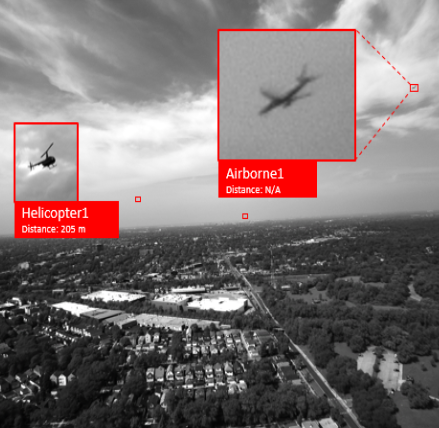
\includegraphics[width=0.5\textwidth]{figures/dataset-example-labeled.png}
        \caption{An example of airborne object dataset}
        \label{fig:airborne-object-example-1}
    \end{figure}
    \vspace{-2ex}
    %Seiring berkembangnya teknologi \emph{autonomous vehicles}, terdapat banyak keinginan untuk mengaplikasikan teknologi tersebut di berbagai bidang.
    %Salah satu aplikasi teknologi ini di bidang komersil adalah \emph{Amazon Prime Air}.
    %\emph{Amazon Prime Air} memanfaatkan \emph{Autonomous Aerial Vehicle} (AAV) untuk melakukan pengantaran barang dari warehouse ke rumah kostumer secara \emph{autonomous} \parencite{prime_air}.
    %Untuk melakukan hal ini, AAV yang digunakan harus mempunyai kemampuan penerbangan \emph{autonomous} yang mumpuni.

    %One of the most critical challenges in designing such a system is the 
    %ability to sense and avoid (SAA) obstacles. Although the airspace in 
    %which AAV operate is relatively sparse, there is still a risk of 
    %encountering static obstacles or airborne objects such as birds or drones.
    %In commercial application, such encounter would result not only in the AAV,
    %but also the item which the AAV carries.
    %Airborne objects pose a particularly difficult challenge as they often appear 
    %unexpectedly and approach rapidly from long distances due to their
    %inherent need for speed in flight.

    Autonomous Aerial Vehicle (AAV) have the potential to significantly impact 
    industries, particularly in commercial delivery. One notable example is Amazon 
    Prime Air, which is currently under development. Prime Air aims to deliver 
    goods from Amazon warehouses directly to customers \parencite{prime_air}. 
    To accomplish this, AAV require a reliable and efficient autonomy system.
 
    One of the most critical challenges in designing an AAV system is the 
    ability to sense and avoid (SAA) obstacles. While the airspace in which 
    AAVs operate may be relatively sparse, there is still risk of encountering 
    static obstacles or airborne objects such as birds or drones. In commercial 
    applications, such encounters can have consequences not only for the AAV 
    itself but also for the items it carries.  Ensuring effective SAA 
    capabilities is essential to mitigate these risks and safeguard both the AAV 
    and the valuable cargo it transports.


    Most SAA system of AAVs includes camera as their primary sensor.
    Cameras provide visual perception to the AAV, real-time, in the form of images. 
    These images must be processed by a computer vision algorithm to identify
    and localize the obstacles in it so that the AAV can estimate their 
    position and plan actions it needs to do to avoid them.
    There are other onboard sensing options such as LiDAR or radar, but cameras
    are more favored due to their lighter weight, cheaper price, 
    and relatively lower energy consumption compared to active sensors. 

    Airborne objects present a particularly challenging problem in SAA as they can 
    appear unexpectedly and approach rapidly from long distances due to their 
    inherent need for speed in flight. For this reason, it is important to detect airborne
    objects while they are still far away. Unfortunately, their far distance cause them 
    to appear very small on images. Figure \ref{fig:airborne-object-example-1} show an
    example of how airborne objects appear on images. In \textcite{aot_docs}, the airborne 
    objects can appear in the range of 4 to 1000 px on a $2048 \times 2448$ px image, that is,
    around 0.00008 - 0.01 \% of the image area.

    For reasons listed above, the computer vision algorithm to be implemented to detect these airborne objects, 
    must be able to detect small objects accurately. And not only that, it also must be able to do it in real-time.
    The fact that AAVs operating environments are outdoors, brings more trouble for the computer
    vision. Outdoor environment brings large complexity and additional variance to the image distribution, 
    making it almost impossible to handcraft feature extractor for it. This is where non-handcrafted
    feature extractors come in handy, particularly the deep learning approaches. Deep learning models
    have shown incredible abilities in handling complex data. Given enough training data, a deep learning
    model can craft itself feature kernels that can extract the objects in an image, despite being subjected
    to complex outdoor environment. For this reason, deep learning models gained prominence in addressing
    these challenges. 
    \begin{figure} [H]
        \centering
        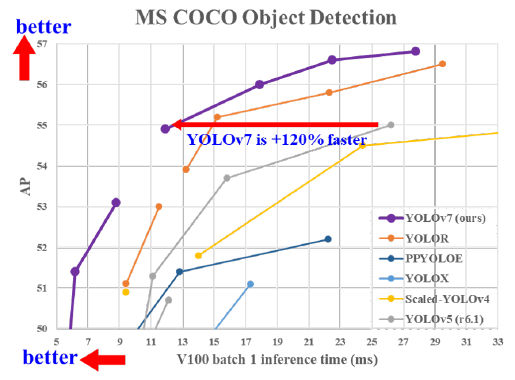
\includegraphics[width=0.75\textwidth]{figures/yolov7-coco.png}
        \caption{YOLOv7 performance on COCO dataset compared to other object detectors.}
        \label{fig:yolov7-coco}
    \end{figure}

    Introducing YOLOv7, a state-of-the-art convolutional neural network based real-time object detector \parencite{yolov7}.
    At the time of the proposal for this research was made (November 2022),
    YOLOv7 outperform both in speed and accuracy of all known real-time object detectors 
    with inference speed in the range of 5-160 FPS. It also has the highest accuracy (56.8\% AP) among
    object detectors with inference speed greater than 30 FPS on a V100 GPU. The capabilities of this cutting-edge architecture
    makes it well-suited for AAV computer vision system. However, all the performance metrics of YOLOv7
    mentioned before are obtained by training the model using COCO 2017 dataset. A dataset which 
    consist of general objects that people see in their daily life. COCO dataset is going to have
    very distinct distribution compared to airborne objects. As such, there would be a need for
    some modification to YOLOv7 so that it could detect airborne objects well.

    The topic of this research is about modifying YOLOv7 with objective of optimizing it to detect
    small objects, which extends to airborne objects. We experimented with some modification to 
    YOLOv7's bag-of-freebies, bag-of-specials, and network architecture. Then we benchmarked the
    modified models against the \textcite{aot_dataset}, and picked the model with the highest AP score
    that can perform inference in real-time.

    %For this to work, the computer vision algorithm must be able to be executed
    %in a real-time scenario, but also must be accurate enough 

    %Introducing YOLOv7. 

    %Dengan memilih kamera sebagai sensor, maka dibutuhkan suatu model computer vision untuk diaplikasikan pada kamera tersebut.
    %Objek - objek \emph{airborne} akan tampak sangat kecil pada kamera seperti yang dapat dilihat pada Gambar \ref{fig:airborne-object-example-1}.
    %Beberapa dataset kamera \emph{airborne} yang memiliki resolusi 20482448 pixel, objeknya dapat berukuran 4 (0.00008\% luas resolusi) hingga 1000 pixel (0.01\% luas resolusi) sehingga terlihat sangat kecil \parencite{aot_dataset}.
    %Oleh karena itu, dibutuhkan suatu model yang dapat mendeteksi objek - objek yang sangat kecil sehingga dapat mendeteksi objek \emph{airborne}.


    %YOLOv7 merupakan model state-of-the-art untuk melakukan pendeteksian objek secara real-time.
    %YOLOv7 memiliki akurasi tertinggi dari semua model pendeteksi objek dengan kecepatan deteksi 30 FPS (yang terpublikasi) pada GPU Nvidia V100.
    %Terdapat versi scaled dari YOLOv7 yang memiliki jumlah parameter yang lebih kecil dan dapat diaplikasikan pada device edge computing \parencite{yolov7}.
    %Oleh karena itu, YOLOv7 ini cocok untuk digunakan pada AAV di mana dibutuhkan suatu pendeteksi objek yang real-time.

\section{Problem Statement}
    
    %YOLOv7 bukan merupakan model deteksi objek umum sehingga YOLOv7 tidak didesain untuk melakukan deteksi objek kecil seperti objek-objek \emph{airborne}.
    %Oleh karena itu, dibuatlah rumusan masalah seperti berikut:
    %\begin{itemize}
    %    \item Apa solusi yang dapat diaplikasikan pada YOLOv7 agar kemampuan deteksi objek \emph{airborne}-nya dapat dioptimalisasi?
    %\end{itemize}
    YOLOv7 is not an object detection model specifically designed to detect small objects or airborne objects.
    Therefore, this research ask the following question.
    \begin{itemize}
        \item What modification can be done to YOLOv7 to improve its abilities in detecting airborne objects?
    \end{itemize}

\section{Purpose}
    The purpose of this research is to find modifications of YOLOv7 that would improve its ability in detecting airborne objects.
    %Adapun tujuan dari tugas akhir ini adalah untuk menemukan solusi untuk mengoptimisasi kemampuan YOLOv7 mendeteksi objek airborne.

\section{Problem Scope}
    % superintelligent AGI
    % solomonoff induction
    In this research, we want to formulate the scope of the problem such that the modifications applied
    on YOLOv7 would not lose its real-time detection ability and is still reasonably computable/trainable.
    Otherwise, we can just run a Solomonoff induction on airborne object data and call the result a modification
    of YOLOv7. Thus, we state the following scopes for the problem.
    \begin{itemize}%[noitemsep,topsep=0pt]
        \item YOLOv7 is used as the baseline for modifications. 
        \item The result of modification must be able to perform inference in real-time.
        \item The modified YOLOv7 must be trainable within a reasonable duration using the computational resource
        available, which is a computer which uses consumer GPU Nvidia RTX 2080 Ti.
    \end{itemize}
    %Optimisasi kemampuan deteksi objek kecil hanya akan dilakukan dengan memodifikasi YOLOv7.
    %Modifikasi yang diaplikasikan tidak boleh menyebabkan YOLOv7 untuk tidak dapat melakukan pendeteksian secara \emph{real time}.
    %Target pengaplikasian model ini adalah untuk AAV dengan \emph{computational resource} yang terbatas sehingga model hasil modifikasi harus cukup ringan untuk hal tersebut.
    %%Modifikasi yang mengubah arsitektur YOLOv7 secara signifikan sehingga tidak dapat melakukan pendeteksian secara \emph{real-time} tidak akan diaplikasian.
  \newpage

  % Konten tinjauan pustaka
  \chapter{LITERATURE REVIEW}
\section{Theoretical Basis}
  \subsection{Object Detection Task}

  Object detection is a fundamental task in computer vision.
  It is a task that have 2 objective, localization and classification.
  Localization is about determining the spatial properties of an object, e.g. by
  enclosing them in bounding boxes. Classification is about determining the class of
  objects if they are animal, human, necromancer, or anything in the set of classes.

  To measure how well an object detection algorithm or model perform, computer vision
  researchers defined metrics to measure how fit a model prediction to an object
  and to measure how well the model perform across all objects. Example of those metrics are IoU and mAP.

  \subsubsection{Intersection Over Union (IoU)}
   \begin{figure}[H]
        \centering
        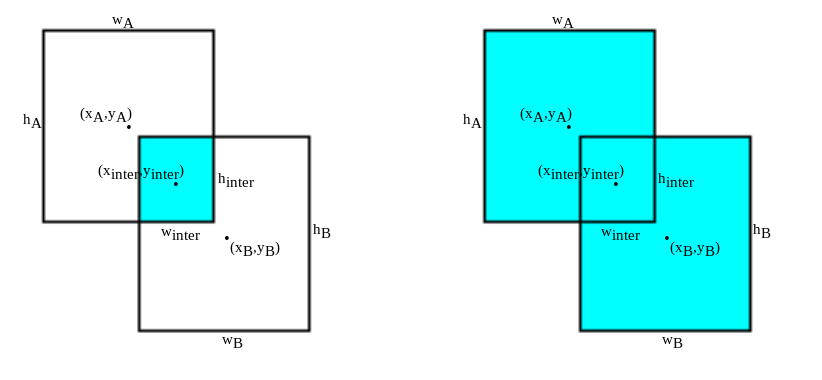
\includegraphics[width=0.7\textwidth]{figures/inter-union.png}
        \caption{Intersection and Union of 2 Bounding Boxes}
        \label{fig:inter-union}
    \end{figure}
  Intersection over union (IoU) is a widely used metrics to determine how fit a predicted bounding box against the true bounding box.
  It is done by calculating the area of the intersection between the predicted and dividing it by the area of the
  union of those 2 boxes. 
  
  The IoU of 2 bounding boxes A and B can be calculated using the following way:
  \begin{itemize}
    \item Calculate the area of intersection of A and B. 

    Let $(x_A,y_A)$ and $(x_B,y_B)$ be coordinates of the center of the box A and B respectively,
    and let $(w_A,h_A)$ and $(w_B,h_B)$ be widths and heights of the center of the bow A and B.

    The calculation for the area of intersection can be done like this:
    \begin{align*}
      x_{\text{{inter}}} &= \max(x_A, x_B) \\
      y_{\text{{inter}}} &= \max(y_A, y_B) \\
      w_{\text{{inter}}} &= \min(x_A + w_A, x_B + w_B) - x_{\text{{inter}}} \\
      h_{\text{{inter}}} &= \min(y_A + h_A, y_B + h_B) - y_{\text{{inter}}} \\
      \text{Area}_{\text{inter}} &= w_{\text{{inter}}} \times h_{\text{{inter}}}
    \end{align*}
    \item Calculate the area of union.

    From set theory, we know that $|A \cup B| =|A| + |B| - |A \cap B| $.
    This also applies when calculating the area of union.
    \begin{align*}
      \text{Area}_{union} &= \text{Area}_A + \text{Area}_B - \text{Area}_{\text{inter}}\\
      \text{Area}_{union} &= w_A\times h_A + w_B\times h_B  - \text{Area}_{\text{inter}}
    \end{align*}
    \item Finaly, calculate IoU
    \begin{equation}
      IoU = \frac{\text{Area}_{\text{inter}}}{\text{Area}_{\text{union}}}
    \end{equation}
  \end{itemize} 

  \subsubsection{Mean Average Percision (mAP)}
  Average Precision (AP) is a popular metrics used to measure the capability of an object detection model
  for a given dataset. The main advantage of using AP are its ability to capture the precision recall
  tradeoff and its independence towards confidence threshold. AP has these 2 advantage as an effect of the way 
  it is calculated.

  To calculate AP, precision and recall area under the curve (AUC) must be calculated first.
  Precision is defined as
  \begin{equation}
    P(\mathbb{S}_c,h,\tau,\epsilon) = \dfrac{\left|\left\{(\hat{B},x) \in \mathbb{S} :\ \exists B \in h(x,\tau)_c,\ IoU(\hat{B},B) > \epsilon  \right\}\right|}{\left| \{B \in h(x,\tau)_c\} \right|}
    \label{eq:precision}
  \end{equation}
  \begin{align*}
    \text{Where}~ h &=  \text{hypothesis/model that predict bounding boxes}\\%\tau}\\
    \mathbb{S}_c &= \text{set of bounding boxes of class $c$ in dataset paired with their respective image}\\
    h(x,\tau)_c &= \text{bounding boxes predicted by $h$ with class $c$}\\
    \tau &= \text{confidence threshold for $h$} \\
    \epsilon &= \text{$IoU$ threshold for a positive prediction}\\
    B &= \text{Bounding box}\\
    x &= \text{image}
  \end{align*}
  and for recall, it is defined as
  \begin{equation}
    R(\mathbb{S}_c,h,\tau,\epsilon) = \dfrac{\left|\left\{(\hat{B},x) \in \mathbb{S} :\ \exists B \in h(x,\tau)_c,\ IoU(\hat{B},B) > \epsilon  \right\}\right|}{\left| \mathbb{S}_c \right|}
    \label{eq:recall}
  \end{equation}
  Then we define the precision recall curve as a parametric function
  \begin{equation}
    PR(\tau) = \left( R(\mathbb{S}_c,h,\tau,\epsilon),P(\mathbb{S},h,\tau,\epsilon) \right)
    \label{eq:pr}
  \end{equation}
  Using equation \ref{eq:pr}, $PR$ curve in Figure \ref{fig:pr-curve} can be generated using $0 \leq \tau \leq 1$
  \begin{figure}[H]
        \centering
        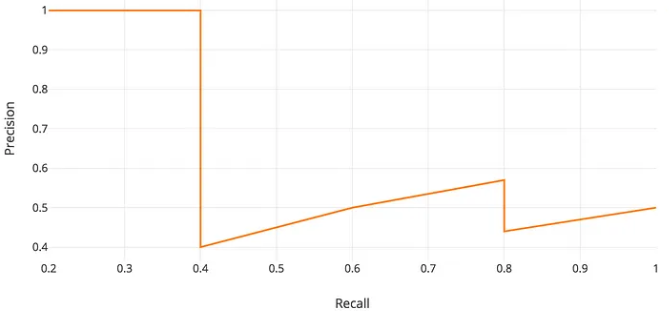
\includegraphics[width=0.75\textwidth]{figures/pr-curve.png}
        \vspace{-1ex}
        \caption*{Source: \textcite{map-hui}}
        \vspace{-1ex}
        \caption{PR Curve Generated by Varying $\tau$}
        \label{fig:pr-curve}
  \end{figure}
  Before calculating the AP however, the curve in Figure \ref{fig:pr-curve} is usually interpolated using Equation \ref{eq:pr-inter},
  which relies on Equation \ref{eq:pr-functionization} that transformed $PR$ curve to a functional relation of R to P.
  The interpolated curve can be seen on \ref{fig:pr-interp}

  \begin{align}
    \label{eq:pr-inter}
    p_{inter}(r) &= \max_{\bar{r}>r} p(\bar{r})\\
    \label{eq:pr-functionization}
    \text{Where}~p(\bar{r}) &= \max \left\{p : \forall (r,p) \in \{PR(\tau) , 0\leq\tau\leq 1\}, r=\bar{r}\right\}%\text{precision given recall value in Figure \ref{fig:pr-curve}}
  \end{align}

  \begin{figure}[H]
        \centering
        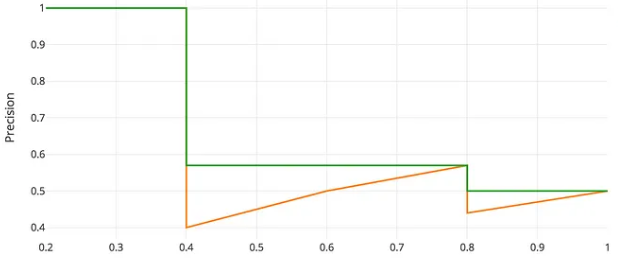
\includegraphics[width=0.75\textwidth]{figures/pr-interp.png}
        \vspace{-1ex}
        \caption*{Source: \textcite{map-hui}}
        \vspace{-1ex}
        \caption{PR Curve Interpolated}
        \label{fig:pr-interp}
  \end{figure}
  The AP, which is the area under the curve then can be calculated using the following integral:
  \begin{equation}
    AP = \int_{0}^{1} p_{inter}(r) \, dr
  \end{equation}

  When calculating AP, the $IoU$ threshold for positive detection is usually predefined. As example,
  for AP@50, we set the $\epsilon$ in Equation \ref{eq:precision} and \ref{eq:recall} to 50\%. And for 
  AP@75, the $\epsilon$ is set to 75\%.

  The AP calculation so far only works for a single class. To have a multiclass metric, we use mAP
  which is calculated as the average AP across all classes in the dataset.
  \begin{equation}
    mAP@X = \frac{1}{|\text{classes}|} \sum_{c\in \text{classes}} AP_c@X
  \end{equation}
  %\begin{align*}
  %  \text{Where}~p(r) &= \text{precision given recall value in Figure \ref{fig:pr-curve}}
  %\end{align*}
  %Traditionally, object detection algorithms relied on handcrafted feature kernels and machine learning techniques. 
  %However, deep learning has become a popular solution for object detection by the use of Convolutional Neural Networks (CNN)
  %to learn feature kernels automatically. With the usage of deep learning, object detection task
  %had significant advancement in terms of accuracy and efficiency.


  \subsection{YOLO Family Architecture}
  YOLO is an abbreviation of "You Only Look Once" which describes what kind of neural network YOLO
  is, a single stage object detector. It means that this architecture predicts regions 
  and classes both at once. In contrast, two-stage detector predicts objects' regions first
  and then predicts their classes. Detecting objects in a single-stage manner is what gave YOLO
  architecture the ability to infer in real-time. This is possible due to how YOLO architecture
  was designed. YOLO architecture consist of 3 main part, the head, the neck, and the backbone.

    %Arsitektur famili YOLO pada dasarnya terbagi akan 3 bagian yaitu \emph{head}, \emph{neck}, dan \emph{backbone}.
    %Setiap bagian ini mempunyai fungsi masing-masing.
   
    %Berikut adalah penjelasan fungsi dan cara kerja dari ketiga bagian tersebut.
    \subsubsection{Backbone}
    The backbone is the network that extract features from the inputted image.
    Typically, the backbone is composed of deep neural network layers that progressively 
    downsample the spatial dimensions of the input while increasing the number of 
    learned features or meaningful abstraction of the data.

    The implementation of backbone in YOLO usually varies from one version to another.
    As example, \textcite{yolov2}'s YOLOv2 implemented Darknet-19 network as backbone, 
    \textcite{yolov3}'s YOLOv3 implemented Darknet-53, \textcite{yolov4}'s YOLOv4
    with their CSP-Darknet-53, or \textcite{vityolo} with their non-CNN (Transformer) backbone.
    Each of these network has their own has their own advantages and disadvantage when
    it comes to accuracy, memory requirement, or latency.


    %\emph{Backbone} dari YOLO merupakan bagian yang mengekstrak fitur dari citra yang diinputkan.
    %Hasil ekstraksi fitur ini akan diinputkan pada \emph{neck} yang kemudian akan di\emph{upsampling} olehnya.
    %Model-model YOLO dapat menggunakan \emph{feature extractor} dari model-model klasifikasi citra sebagai \emph{backbone}-nya.
    %Sebagai contoh, salah satu varian YOLO, YOLO-Z menggunakan DenseNet sebagai \emph{backbone}-nya sedangkan arsitektur YOLO dasarnya, YOLOv5 menggunakan \emph{backbone} YOLOv5v7.0 \parencite{yoloz}.
    \subsubsection{The Neck}
  
    \begin{figure}[H]
        \centering
        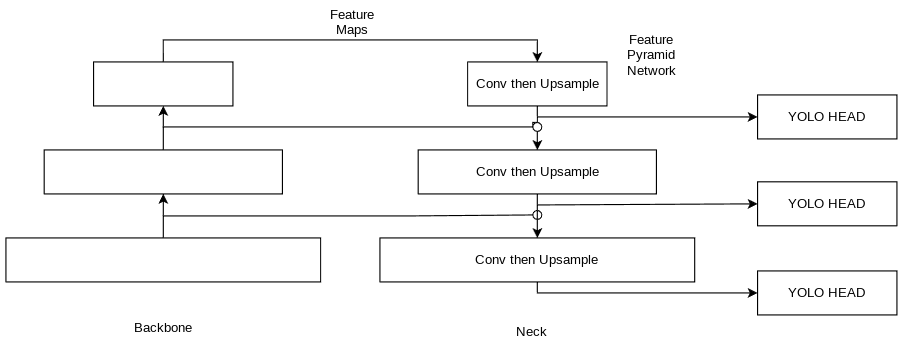
\includegraphics[scale=0.6]{figures/yolo-architecture-rough.png}
        \caption{Feature Pyramid Network in YOLOv3}
        \label{fig:yolofpn}
    \end{figure}

    The neck is the intermediate network between backbone and head.
    The main function of the neck is to enhance features extracted by the backbone.
    Specific implementation of neck for each YOLO architecture is different one to the other.
    Some neck implementation try to combine feature maps across different prediction scales of YOLO network.

    \textcite{yolov3} was the first to introduce YOLO prediction in multiple scale in YOLOv3.
    To enhance the feature maps with using information across scales, YOLOv3 fuses features 
    from multiple parts of the backbone before up sampling them as seen on Figure \ref{fig:yolofpn}. 
    This type of neck network is called Feature Pyramid Network (FPN). 
    A further improvement was made by \textcite{yolov4} with their YOLOv4 by introducing Path 
    Aggregation Network (PANet) for the neck. 
    With PANet, feature are fused back to higher scale by adding another FPN-like layer after the original FPN
    but with reverse direction.
    %The way it works is by taking feature maps, not only in the last output layer of the
    %backbone, but also in multiple parts of the backbone.
    %For example, YOLOv4 uses PANet to enhance and combine features across different scales
    %of prediction.
  
    %\emph{Neck} dari YOLO merupakan \emph{layer-layer} dimana \emph{head} YOLO mengambil fitur untuk dilakukan deteksi \emph{bounding box}.
    %Pada YOLOv3 \textcite{yolov3}, arsitektur \emph{neck} dibuat menyerupai \emph{Feature Pyramid Network} (FPN) seperti pada Gambar \ref{fig:yolofpn}. 
    %Pada versi-versi YOLO selanjutnya, bentuk \emph{neck} ini tidak banyak berubah dan pada dasarnya tetap mempertahankan bentuk \emph{pyramid}-nya.
  
    %Penaikkan tingkatan \emph{pyramid} dari FPN merupakan \emph{upsampling} dari \emph{feature map} yang dihasilkan \emph{backbone}.
    %Output tiap tingkatan pada FPN di \emph{neck} inilah yang diinputkan pada \emph{head} YOLO. 
    %Melakukan prediksi pada tingkatan \emph{upsampling} yang berbeda-beda dapat membuat \emph{neural network} mendapatkan lebih banyak informasi semantik dan informasi yang lebih detail sehingga dapat lebih akurat dalam mendeteksi objek besar maupun kecil.
 

  
    \subsubsection{The Head and The Anchors}
    \begin{figure}[H]
        \centering
        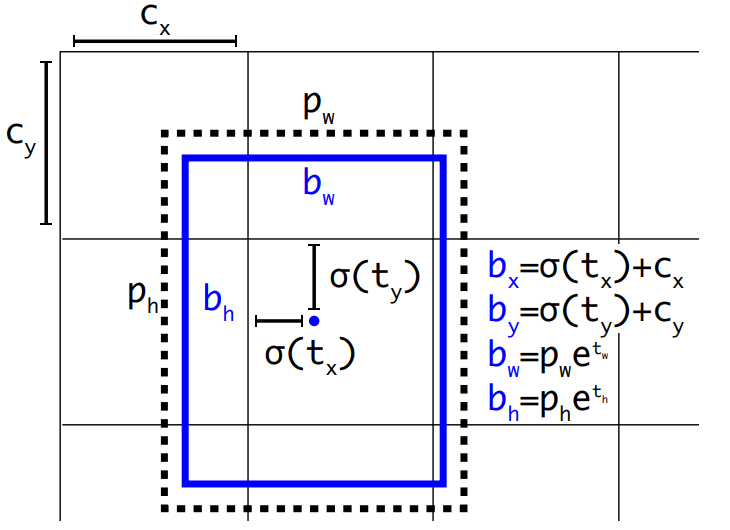
\includegraphics[width=0.5\textwidth]{figures/anchorbox.png}
        \caption*{Source: \textcite{yolov3}}
        \caption{Head layer predict anchor box and its offsets from lattice of the feature grid }
        \label{fig:anchorbox}
    \end{figure}
    The head is where the object detection happens. Extracted and enhanced features of the image is fed to the head 
    in multiple different scales. For each scale, the head will predict a box for each $N \times N$
    lattice point on feature map's grid. In total, each layer will output a tensor with size
    $N_k \times N_k \times [A_k \times (4+1+C)]$ where $N_k$ is the size of feature map grid at the $k$-th scale,
    $A_k$ is the number of anchors for that scale, 4 is for the four offsets $[t_x, t_y, t_w, t_h]$ in figure 
    \ref{fig:anchorbox}, 1 is for the objectness score for the grid, and $C$ is for the number of classes it has
    to predict.
    
    Most of YOLO family architecture head utilizes anchor boxes to assist bounding box prediction.
    This technique is used in \textcites{yolov2}{yolov3}{yolov4}{scaledyolov4}{yolov5}{yolor}{yolov7}.
    Instead of directly predicting the size and position of the bounding box, YOLO head predicts 
    the offsets for each anchor boxes assigned to the head, then it utilizes the objectness score to pick
    which result  of these anchor boxes to be used.
    Using anchor boxes allows the neural network to converge more quickly because it provides
    a prior knowledge of the dataset before training.
    
    %The way it works is that, there will be a preset of detection boxes.
    %Arsitektur famili YOLO yang dipublikasikan setelah YOLOv2 terus menggunakan \emph{anchor box} untuk melakukan deteksi \parencites{yolov2}{yolov3}{yolov4}{scaledyolov4}{yolov5}{yolor}{yolov7}.
    %\emph{Anchor boxes} merupakan beberapa \emph{Bounding Box} yang telah terdefinisikan. 
    %Arsitektur YOLO akan memprediksi probabilitas \emph{anchor box} berada pada suatu koordinat latis beserta dengan \emph{offset anchor box} tersebut untuk menepatkan \emph{anchor box} pada objek yang dideteksi.
    %Penggunaan \emph{anchor box} ini dapat meningkatkan akurasi deteksi karena \emph{neural network} hanya perlu mencari titik tengah objek dan \emph{error} dimensi \emph{boudning box} dengan menggunakan \emph{offset} \parencite{yolov3}.
    %Hal ini lebih sederhana daripada mencari titik-titik \emph{bounding box} secara independen sehingga lebih mudah untuk dipelajari oleh \emph{neural network}.
  
    %Prediksi \emph{bounding boxes} terjadi di bagian \emph{head} dari arsitektur YOLO.
    %Bagian \emph{head} dari YOLO akan mengambil beberapa hasil \emph{upsampling} yang terjadi pada \emph{neck} YOLO, dan kemudian melakukan prediksi \emph{anchor boxes} dari hasil tersebut.
    %Hasil prediksi \emph{Head} YOLO pada suatu tingkatan \emph{upsampling} berupa tensor dengan ukuran $N\times N \times [A\times(4+1+C)]$ dengan $N$ sebagai dimensi hasil \emph{upsampling}-nya, $A$ sebagai jumlah \emph{anchor boxes} untuk \emph{scaling} tersebut, dan $C$ sebagai jumlah kelas prediksi.
    %Angka 4 merepresentasikan 4 \emph{offset} $b_x, b_y, b_w, b_h$ seperti pada Gambar \ref{fig:anchorbox} dan angka 1 merepresentasikan \emph{objectness score} dari prediksi \emph{bounding box}.

    \subsubsection{Loss Function}
    The goal of a YOLO architecture is to (1) predict if an object exist or not, (2) predict the bounding box of such object,
    and (3) predict the class of the object. These 3 loss functions that correspond to those objectives are called 
    objectness loss, box loss, and class loss respectively. To update the weights on training, the total loss is calculated as 
    the weighted sum of those 3 losses.
    %\begin{equation}
    %  L_{box} = \sum_{k=0}^{n}\sum_{i,j=0}^{N_k}\sum_{m=0}^{A_k} \mathbbm{1}_{k,i,j,m}^{obj} -IoU(gt(x), M(x)_{k,i,j,m})
    %\end{equation}
    In original YOLO, the loss functions were defined like the following.

    For localization loss, it is described by equation \ref{eq:yolo-box-loss}.
    \begin{equation}
      L_{box} = \sum_{i=0}^{S^2} \sum_{j=0}^B \mathbbm{1}_{ij}^{obj} \left[(x_i - \hat{x}_i)^2 + (y_i - \hat{y}_i)^2 + (\sqrt{w_i}-\sqrt{\hat{w}_i})^2 + (\sqrt{h_i}-\sqrt{\hat{h}_i})^2\right] \\
      \label{eq:yolo-box-loss}
    \end{equation}
    \begin{align*}
    \text{Where}~S^2  &= \text{the total number of grid cells in the output,}\\
    B &= \text{ the total number of anchor box per grid cells,}\\
    \mathbbm{1}_{ij}^{obj} &= \begin{cases}
                                1, & \text{if object present in grid}\\
                                0, & \text{otherwise,}
                              \end{cases} 
                              \\
    (x_i, y_i) &= \text{the predicted coordinates of the center of object i}\\
    (\hat{x}_i, \hat{y}_i) &= \text{the ground truth coordinates of the center of object}\\
    (w_i, h_i) &= \text{the predicted width and height of object i}\\
    (\hat{w}_i, \hat{h}_i) &= \text{the ground truth width and height of object}
      %\text{the indicator variable that has value 1 if object is present in the grid and 0 otherwise.}
    \end{align*}
    %$\mathbbm{1}_{ij}^{obj}$ is the indicator variable that has value 1 if object is present in the grid and 0 otherwise.
    %$(x_i, y_i)$ and $(\hat{x}_i, \hat{y}_i)$ are the predicted and ground truth coordinates of the center of object $i$.
    %$(w_i, h_i)$ and $(\hat{w}_i, \hat{h}_i)$ are the predicted and ground truth widths and heights of object $i$.
    For objectness loss, described by equation \ref{eq:yolo-obj-loss}
    \begin{equation}
      L_{obj} = \sum_{i=0}^{S^2} \sum_{j=0}^B \mathbbm{1}_{ij}^{obj}(C_i - \hat{C}_i)^2  + \alpha \mathbbm{1}_{ij}^{noobj}(C_i - \hat{C}_i)^2
      \label{eq:yolo-obj-loss}
    \end{equation}
    \begin{align*}
    Where~\mathbbm{1}_i^{\text{noobj}} &=\begin{cases} 
                                          1, & \text{if object assigned to anchor j}\\
                                          0, & \text{otherwise} 
                                         \end{cases}\\
          (C_i,\hat{C}_i) &= \text{predicted and ground truth confidence score for objectness of anchor}
    \end{align*}
    %$(C_i, \hat{C}_i)$ are the predicted and ground truth confidence scores for objectness of anchor $i$,
    And for class loss, described by \ref{eq:yolo-class-loss}
    \begin{equation}
      L_{class} = \sum_{i=0}^{S^2} \mathbbm{1}_{ij} \sum_{c \in classes} (p_i(c) - \hat{p}_i(c))^2
      \label{eq:yolo-class-loss}
    \end{equation}
    Where $(p_i(c), \hat{p}_i(c))$ are the predicted and ground truth class probabilities for class $c$ for object $i$.

    The three losses combined to the final loss function in equation \ref{eq:yolo-loss}
    \begin{equation}
      L = \lambda_{box}L_{box} + \lambda_{obj}L_{obj} + \lambda_{class}L_{class}
      \label{eq:yolo-loss}
    \end{equation}
    \begin{align*}
      Where~\lambda_{box} &= \text{the weight for localization,}\\
      \lambda_{obj} &= \text{weight for objectness}\\
      \lambda_{class} &= \text{weight for class}
    \end{align*}
    These 3 $\lambda$-s can be tuned to optimize the performance of a YOLO network.

    %\begin{equation}
    %  L_{box} = \sum_{i=0}^{S^2}\sum_{j=0}^B   \mathbbm{1}_{ij}^{obj} (x_i-\hat{x}_i)^2 + (y_i-\hat{y}_i)^2 + (\sqrt{w_i}-\sqrt{\hat{w}_i})^2 + (\sqrt{h_i}-\sqrt{\hat{h}_i})^2 
    %\end{equation}
      %L_{box} = \sum_{k=0}^{n}\sum_{i,j=0}^{N_k}\sum_{m=0}^{A_k} \mathbbm{1}_{k,i,j,m}^{obj} -IoU(gt(x), M(x)_{k,i,j,m})

    %\begin{equation}
    %  L_{box} = 1
    %\end{equation}

  
      
  \subsection{YOLOv7}
  As said in section \ref{section:background}, YOLOv7 is the state-of-the-art real-time object detector.
  It was made by the authors of YOLOv4, and by the time it was published (july 2022), it surpassed all 
  known real-time object detectors both in speed and accuracy. To achieve this, YOLOv7 implemented some new
  changes and addition to the neural network. 
  \subsubsection{Backbone}

%  \vspace{-2ex}
  %\begin{figure}[H]
  %    \centering
  %    \subfigure[ELAN block]{
  %    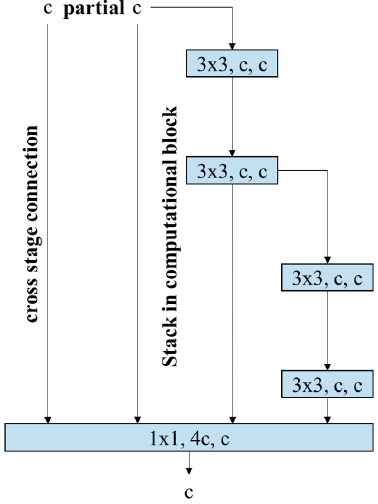
\includegraphics[width=0.2\textwidth]{figures/elan-block.png}
  %    \label{fig:elan-block}
  %    }
  %    \subfigure[FIGTOPCAP][First two ELAN blocks in YOLOv7]{
  %    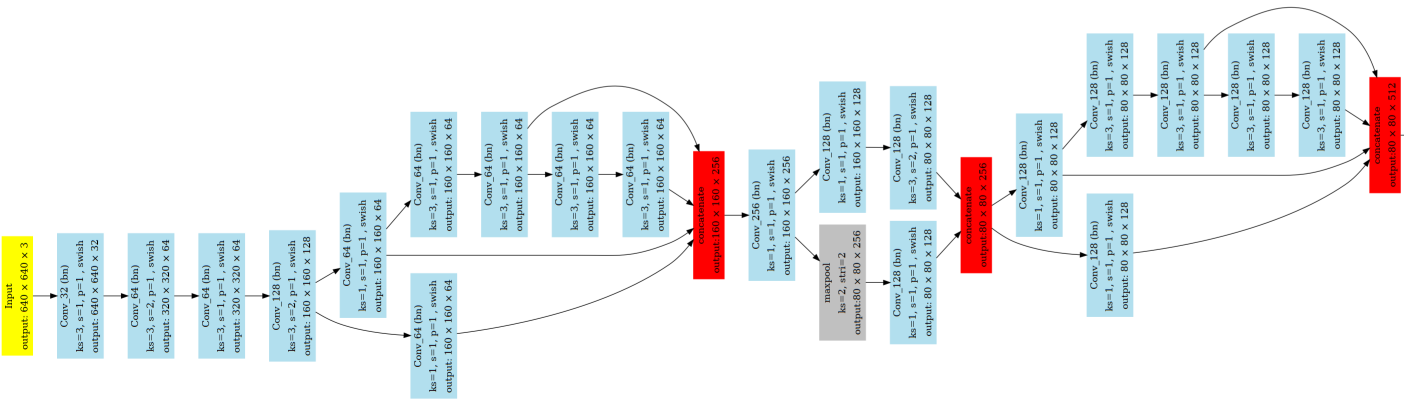
\includegraphics[width=0.75\textwidth]{figures/yolo-elan-blocks.png}
  %    \label{fig:elan-yolo}
  %    }
  %    \caption{ELAN in YOLOv7}
  %    \label{fig:elan}
  %\end{figure}
  \begin{figure}[H]
    \centering
    \begin{subfigure}[c][][c]{.35\textwidth}
        %%%\vspace{0pt}
        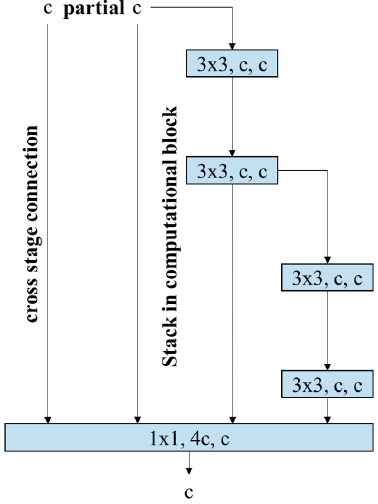
\includegraphics[width=1\linewidth]{figures/elan-block.png}
        \caption{ELAN block}
        \label{fig:elan-block}
    \end{subfigure}

    \begin{subfigure}[c][][c]{.9\textwidth}
        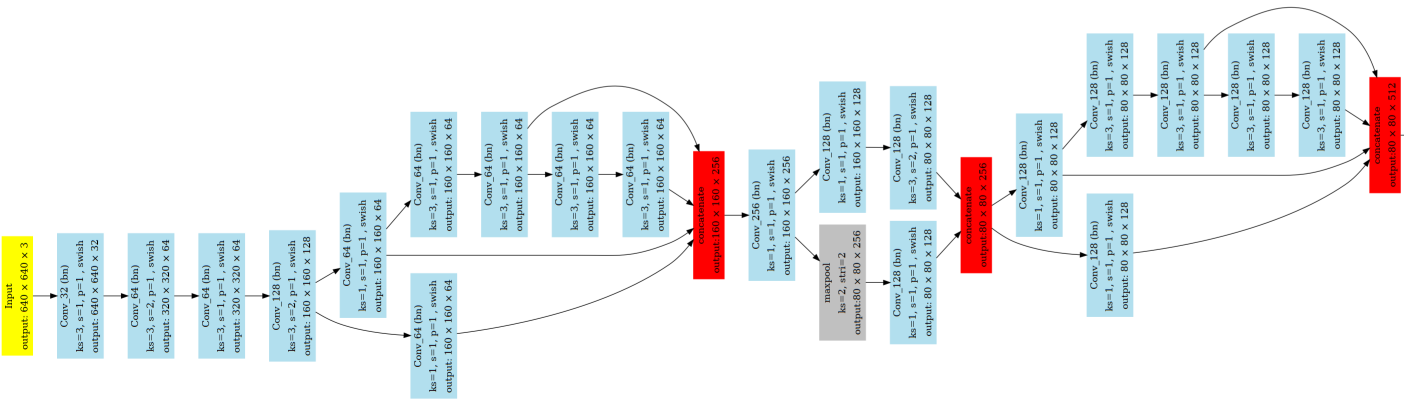
\includegraphics[width=1\linewidth]{figures/yolo-elan-blocks.png}
        \caption{First two ELAN blocks in YOLOv7}
        \label{fig:elan-yolo}
    \end{subfigure}
    \caption*{Source: \textcite{yolov7}}
    \caption{ELAN in YOLOv7}
    \label{fig:elan}
  \end{figure}

  %remove this negative vspace if buku TA kurang panjang

  YOLOv7 implemented the Efficient Layer Aggregation Network (ELAN) and Extended-ELAN (E-ELAN) as the backbone of its network. 
  ELAN is a convolutional neural network that was designed to extract features efficiently 
  by controlling the shortest longest gradient path in the network \parencite{elan}.
  This choice of backbone allows YOLOv7 to perform prediction more accurately despite having fewer number of parameters. 
  Figure \ref{fig:elan-yolo} shows how ELAN block in Figure \ref{fig:elan-block} implemented in YOLOv7.

  \subsubsection{Label Assignment Strategy and Auxilary Head}
  \begin{figure}[H]
      \centering

      \begin{subfigure}[][][t]{0.5\textwidth}
        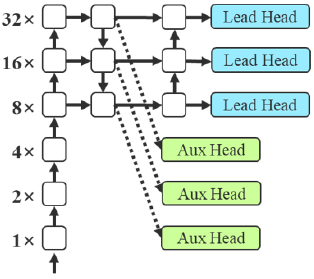
\includegraphics[width=1\linewidth]{figures/auxilary-head.png}
        \caption{Auxliary heads attachment in YOLOv7}
        \label{fig:aux-head}
      \end{subfigure}

      \begin{subfigure}[][][t]{0.4\textwidth}
        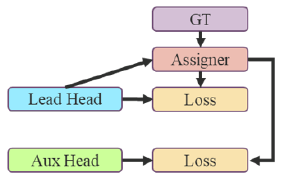
\includegraphics[width=1\linewidth]{figures/lead-head-assigner.png}
        \caption{Lead guided label assignment}
        \label{fig:lead-head}
      \end{subfigure}\hfill
      \begin{subfigure}[][][t]{0.4\textwidth}
        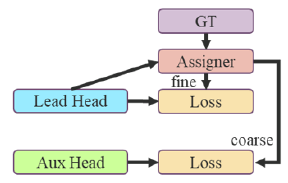
\includegraphics[width=1\linewidth]{figures/coarse-to-fine.png}
        \caption{Coarse-to-fine lead guided label assignment}
        \label{fig:coarse-to-fine}
      \end{subfigure}
      \caption*{Source: \textcite{yolov7}}
      \caption{YOLOv7 Label Assignment Strategy with Auxilary Heads}
      \label{fig:labelassigner}
  \end{figure}
  SimOTA, first introduced in YOLOX, is an algorithm to approximate Optimal Transport Assignment (OTA)
  in a faster way. \textcite{yolox} introduced SimOTA in YOLOX because OTA was deemed too slow to compute
  as it was increasing the training time by 25\%. YOLOv7 also implemented SimOTA for its dynamic label assigner.

  YOLOv7 deep supervised its training process by attaching auxilary heads to its neural network
  as seen on Figure \ref{fig:aux-head}.
  These auxilary heads is only used on training, on inference, they are removed from the neural network
  to improve latency, only the lead head is kept. There is a problem however with assigning labels
  to the auxilary and lead heads. Most object detection networks that utilizes auxilary heads have 2
  independent label assigners, one for auxilary heads and one for lead heads. YOLOv7 done things differently.


  YOLOv7 proposed 2 way of assigning labels to auxilary and lead heads. Lead head guided label assignment (Figure \ref{fig:lead-head}) and
  coarse-to-fine lead head guided assignment (Figure \ref{fig:coarse-to-fine}). For lead head guided label assignment, the assigner gives a copy
  of lead heads' label assignment to the auxilary heads. For coarse-to-fine lead head guided assignment, the 
  assigner works like lead head guided assigner but gives coarse label assignment to auxilary head. Coarse label
  assignment is done by relaxing the positive sample constraints of the assigner. \textcite{yolov7} find that coarse-to-fine
  label assignment produces the greatest AP scores.
  
  Due to the relaxed constraints, coarse label assignment to auxilary heads assigns more positive labels the auxilary heads' grids. 
  This way, the network will learn more to recall.
  On inference, this recall ability would be filtered by the lead head to produce accurate prediction.

  \subsubsection{Reparameterization}
  YOLOv7 utilized RepConv and YOLOR implicit layers in its network.
  In addition to that, YOLOv7 also uses Convolution-BatchNorm layer.
  These layers can be reparameterized after training to simplify the neural network, thereby reducing
  latency and memory usage but not hurting inference performance.

  The reparameterization of YOLOR implicit layers can be done after training by computing
  some mathematical simplification of the implicit layers.
  For combination of YOLOR\textsuperscript{+}--Convolution--YOLOR\textsuperscript{+} layers, it can be reparameterized like the following.
  \begin{align*}
    x_{n+1} &= W(x_{n}+g_1(z_1)) + b + g_2(z_2)\\
    &= W(x_{n}) + (W(g_1(z_1)) + b + g_2(z_2))\\
    &= W(x_{n}) + b'
  \end{align*}
  Observe that the reparameterization combined 3 layers into a single convolution layer with bias. Then, For combination of
  YOLOR*--Convolution--YOLOR* layers:
  \begin{align*}
    x_{n+1} &= (W(g_1(z_1)x_n)+b)g_2(z_2)\\
    &= g_2(z_2)g_1(z_1)W(x_n) + b g_2(z_2)\\
    &= W'(x_n) + b'
  \end{align*}
  And finally for Convolution-BatchNorm:
  \begin{align*}
    x_{n+1} &= ((W(x_n)+b)-m)/s\\
    &= (W(x_n) + (b-m))/s\\
    &= (W/s)(x_n) + (b-m)/s\\
    &= W'(x_n) + b'
  \end{align*}

  In summary, YOLOR\textsuperscript{+}--Conv--YOLOR\textsuperscript{+} will be replaced with the original convolutional layer $W$ but with bias $W(g_1(z_1)) + b + g_2(z_2)$.
  YOLOR*--Conv--YOLOR* layers will be replaced with a convolutional $g_2(z_2)g_1(z_1)W$ and bias $b g_2(z_2)$.
  And Conv--BatchNorm will be replaced with a convolutional $W/s$ and bias $(b-m)/s$.
  %TODO: reparam equation here
    %YOLOv7 merupakan pendeteksi objek \emph{real time} dengan skor akurasi tertinggi pada dataset COCO di tahun 2022.
    %Pada YOLOv7, dilakukan beberapa perubahan untuk meningkatkan akurasi dan kecepatan deteksinya.
    %Perubahan-perubahan tersebut dilakukan pada arsitekturnya dan pada \emph{bag-of-freebies}-nya.
  
    %Perubahan arsitektur dilakukan pada \emph{backbone}. YOLOv7 menggunakan \emph{Extended Efficient Layer Aggregation Network} (E-ELAN) sebagai \emph{backbone}, berbeda dengan leluhurnya YOLOv4 yang menggunakan CSP-Darknet.
    %E-ELAN merupakan arsitektur \emph{neural network} yang efisien karena E-ELAN didesain dengan mengontrol \emph{gradient path} terpanjang yang terpendek.
    %Karena efisiensinya, arsitektur E-ELAN ini dapat meningkatkan kecepatan deteksi dan akurasi. \parencite{yolov7}
  
    %\emph{Bag-of-freebies} merupakan kumpulan metode peningkatan akurasi yang tidak meningkatkan \emph{cost inferrence} \parencite{yolov4}. 
    %Pada YOLOv7, ditambahkan beberapa \emph{bag-of-freebies} yang dapat dilatih seperti \emph{re-parameterized convolution} dan \emph{extra auxilary head} di tengah-tengah \emph{neural network}.
    %Selain kedua itu, YOLOv7 juga menambahkan \emph{trainable bag-of-freebies} dari YOLOR seperti EMA, \emph{Implicit Knowledge}, dan \emph{conv-bn topology Batch Normalization} \parencite{yolov7}.
    %Introducing YOLOv7, a state-of-the-art deep learning based real-time object detector \parencite{yolov7}.
    %At the time of the proposal for this research was made (November 2022),
    %YOLOv7 outperform both in speed and accuracy of all known real-time object detectors 
    %with inference speed in the range of 5-160 FPS. It also has the highest accuracy (56.8\% AP) among
    %object detectors with inference speed greater than 30 FPS on a V100 GPU. The capabilities of this cutting-edge architecture
    %makes it well-suited for AAV computer vision system. However, all the performance metrics of YOLOv7
    %mentioned before are obtained by training the model using COCO 2017 dataset. A dataset which 
    %consist of general objects that people see in their daily life. COCO dataset is going to have
    %very distinct distribution compared to airborne objects. As such, there would be a need for
    %some modification to YOLOv7 so that it could detect airborne objects well.


  \subsection{Anchor Recalculation}
  \label{section:anchor_recalc_study}
  Anchor recalculation is a common method of introducing prior distribution of the dataset to an anchor-based object
  detection networks. Most of the time, anchors provided by pretrained YOLO weights are optimized for the common metrics
  dataset such as COCO2017 or VOC2012. Thus, recalculating anchor can help the neural network learn faster.

  There are multiple ways of recalculating anchors. Some of them can be performed before training or during training.
  Most of pre-training anchor recalculation method involves with clustering the anchors to the dataset. This is done by
  using clustering algorithm such as K-means, Gaussian Mixture, and many others. Recalculating anchor on training is 
  a little more complex to do as it will involve some loss function or architectural change on the object detection neural network.
  \textcite{anchoropt} for example add additional layer on detection part of object detectors that is connected to anchor modifiers such that
  the anchors will also be updated during training. \textcite{yolor} mentioned that the implicit multiplication layer of their network
  can be purposed for anchor refinement.

  %\emph{Anchor box} dari model-model \emph{pre-trained} YOLO pada umumnya mengoptimisasi \emph{anchor box} modelnya pada dataset COCO.
  %Ukuran \emph{anchor box} yang akan digunakan pada model YOLO dapat dikonfigurasikan agar lebih sesuai dengan dataset yang akan digunakan untuk melatih model YOLO.
  %Penyesuaian ini dapat meningkatkan IoU(\emph{Intersection Over Union}) prediksi model dengan \emph{ground truth} sehingga meningkatkan akurasi.

  %Penyesuaian anchor box dapat dilakukan pada saat sebelum training atau pada saat training.
  %Penyesuaian anchor box sebelum training dapat dilakukan dengan cara mengkonfigurasi secara manual tiap ukuran \emph{anchor box} atau dengan menggunakan algoritma \emph{clustering}.
  %Penggunaan algoritma \emph{clustering} akan lebih baik karena setiap ukuran \emph{anchor box}-nya disesuaikan dengan pengelompokan-pengelompokan ukuran \emph{bounding box} natural yang terdapat pada dataset.
  %Untuk penyesuaian saat training, dapat digunakan algoritma dari \textcite{anchoropt}.
  %Algoritma ini akan mengoptimisasi ukuran-ukuran anchor bukan hanya berdasarkan dataset, namun berdasarkan kemampuan dari neural network pendeteksi objeknya.
  %Untuk melakukan hal tersebut, algoritma ini akan memanfaatkan back propagation localization loss untuk rekalkulasi anchor.

  \subsection{Mosaic Augmentation}
  \label{section:mosaic_study}
  \begin{figure}[H]
    \centering
    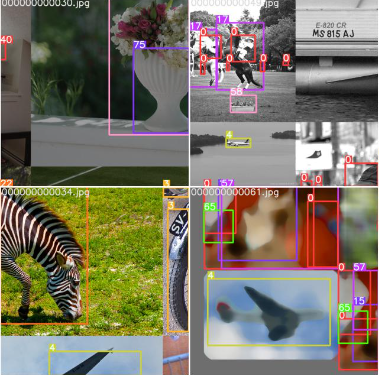
\includegraphics[width=0.5\textwidth]{figures/mosaic-aug.png}
    \caption*{Source: \textcite{yolov5}}
    \caption{Four example of mosaic augmentation \parencite{yolov5}}
    \label{fig:mosaic}
  \end{figure}
  Mosaic augmentation was introduced in Ultralytics' implementation of YOLOv3 \parencite{mosaic_aug}.
  This augmentation technique will randomly pick 4 images of the dataset, and tile them randomly into one image like in \ref{fig:mosaic}.
  It's called mosaic due to how the result of the augmented image have mosaic-like appereance.
  \textcites{cspnet}{yolov4}{yolov5} reported increase in accuracy after applying mosaic augmentation.
  %Augmentasi mosaik merupakan teknik augmentasi yang baru dikenalkan pada YOLOv4.
  %Teknik augmentasi ini akan memilih 4 gambar dari dataset, memotong gambar-gambar tersebut dan menggabungkannya secara acak pada satu gambar seperti pada Gambar \ref{fig:mosaic}.
  %Hasil dari penggabungan itu membuat gambar terlihat seperti mosaik.
  %Teknik augmentasi ini mampu meningkatkan akurasi model \parencite{yolov4}.


\section{Related Works}
\label{section:relatedwork}

  \subsection{YOLO-Z}
  \begin{figure}[H]
    \centering
    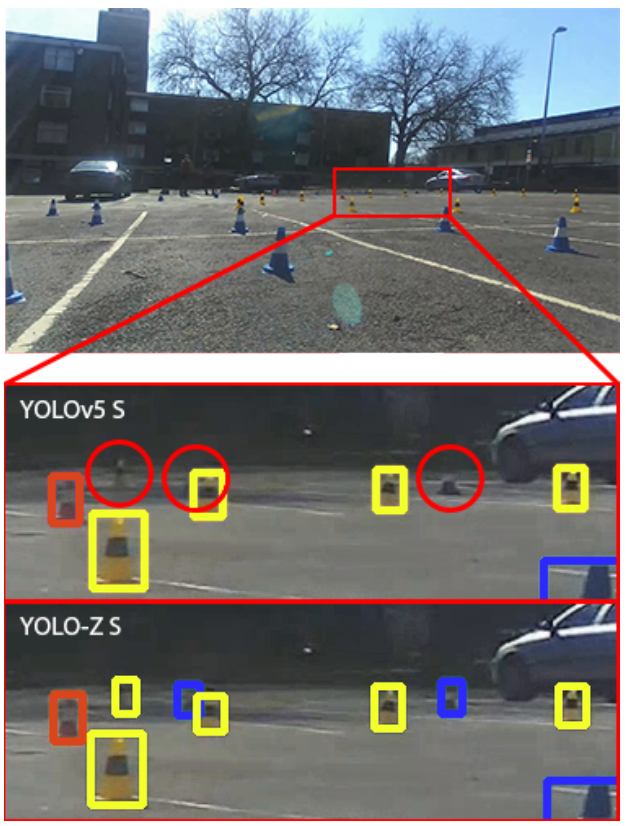
\includegraphics[width=.7\textwidth]{figures/yoloz-result.png}
    \caption*{Source: \textcite{yoloz}}
    \caption{Small objects in the image. Comparison of YOLOZ-S and YOLOv5-S. YOLOv5-S was not able to detect the circled objects.}
    \label{fig:yolozcone}
  \end{figure}
  YOLO-Z is a derivative architecture of YOLOv5r5.0.
  This variant of YOLO modified the backbone, neck, and number of anchors of the original YOLOv5 to 
  enhance its capability of detecting small objects \parencite{yoloz}.
  These changes are backbone change from YOLOv5r5.0 to a downscaled DenseNet,
  neck change from FPN to biFPN on some YOLO-Z scales, and increasing the number of anchors used at each scale.

  YOLO-Z was aimed to be used in autonomous racing car. In this high speed environment, early detection
  of obstacle is crucial to plan for action. For that reason, the autonomous racing car must detect the cone-shaped obstacles
  that are far away from it. Since objects that are far away appear small on image captured by camera, YOLOv7 was designed with
  purpose of small object detection.
  %YOLO-Z merupakan arsitektur famili YOLO yang modifikasi dari YOLOv5 \parencite{yoloz}.
  %Modifikasi-modifikasi yang dilakukan meliputi pergantian \emph{backbone}, \emph{neck}, dan jumlah \emph{anchor}
  %\emph{Backbone} dari YOLOv5r5.0 menjadi DenseNet yang di-\emph{downscale}.
  %\emph{Neck} dari YOLO-Z juga diganti dari PanNet menjadi FPN dan biFPN tergatung pada \emph{scale} YOLO-Z yang digunakan.

  %Modifikasi pada YOLO-Z didesain untuk mendeteksi objek kecil untuk tujuan melakukan deteksi \emph{cone} yang nampak jauh pada lintasan \emph{autonomous racing} secara \emph{real time} (lihat Gambar \ref{fig:yolozcone}).
  %Modifikasi-modifikasi dibuktikan dapat meningkatkan kemampuan pendeteksian objek kecil \parencite{yoloz}.
  %Oleh karena itu, untuk meningkatkan kemampuan mendeteksi objek kecil YOLOv7, beberapa modifikasi yang dilakukan YOLO-Z pada YOLOv5 dapat diaplikasikan.

  \subsection{exYOLO}
  \begin{figure}[H]
    \centering
    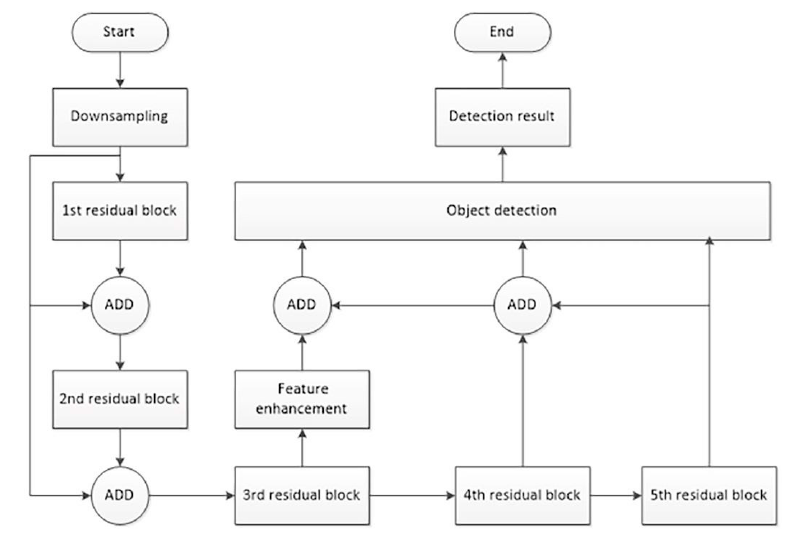
\includegraphics[width=0.8\textwidth]{figures/exyolo.png}
    \caption*{Source: \textcite{exyolo}}
    \caption{Architecture of exYOLO}
    \label{fig:exyolo}
  \end{figure}

  exYOLO is a modification of YOLOv3 to detect small objects \parencite{exyolo}.
  \textcite{exyolo} thought that the features of small objects in an image would disappear
  after series stage of down-sampling in the neural network.
  To solve this exYOLO added a feature enhancement before feature-fusion in the neck to one of the feature scale as seen in Figure \ref{fig:exyolo}.
  This change made exYOLO produce a higher mAP score on VOC2007 compared to its baseline YOLOv3.
    %exYOLO merupakan hasil modifikasi arsitektur YOLOv3 \parencite{exyolo}.
    %Pada exYOLO, dilakukan modifikasi \emph{neck} dengan menambahkan suatu \emph{Receptive Field Block} sebelum penggabungan \emph{feature map} yang akan diupsampling.
    %Modifikasi-modifikasi ini membuat exYOLO memiliki skor mAP yang lebih tinggi daripada YOLOv3 pada dataset PASCAL VOC 2007.

  \subsection{YOLOv4-tiny with added head}%Implementasi YOLOv4-tiny pada \emph{Autonomous Surface Vehicle}}
  \begin{figure}[H]
    \hfill%
    \begin{subfigure}[c][][c]{.45\textwidth}
        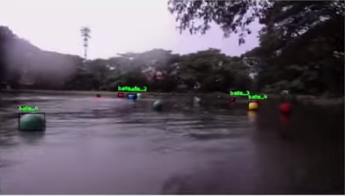
\includegraphics[width=1\linewidth]{figures/yolov4barun-regular.png}
        \caption{Regular YOLOv4-tiny prediction}
        \label{fig:barun-yolov4}
    \end{subfigure}\hfill  
    \begin{subfigure}[c][][c]{.45\textwidth}
        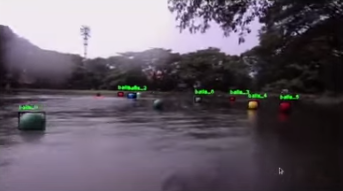
\includegraphics[width=1\linewidth]{figures/yolov4barun-addhead.png}
        \caption{YOLOv4-tiny with added head prediction}
        \label{fig:barun-yolov4-3l}
    \end{subfigure}\hfill%
    \caption*{Source: \textcite{barunastra}}
    \caption{Comparison of regular YOLOv4-tiny and YOLOv4-tiny with added head}
    \label{fig:barun}
  \end{figure}

  \textcite{barunastra} used YOLOv4-tiny as their Autonomous Surface Vehicle (ASV) object detector due to the computational
  device constraint.
  To detect objects that were atleast 30 meters away from the ASV, they applied a modification of YOLOv4-tiny, which was YOLOv4-tiny
  but with additional head layer. The original YOLOv4-tiny only had 2 head layers, thus was only predicting in 2 scales.
  An addition of head layer allows it to predict in 3 scales. Using this modification, the network was able to detect small object
  better and raised the overall mAP score by 4\% without significantly reducing latency.

  %\textcite{barunastra} menggunakan model modifikasi YOLOv4-tiny pada \emph{Autonomous Surface Vehicle}(ASV) mereka.
  %YOLOv4-tiny sebenarnya hanya menggunakan 2 layer head, namun yang diimplementasikan pada ASV adalah model YOLOv4-tiny
  %yang ditambahkan 1 layer head lagi sehingga menggunakan total sebanyak 3 layer head. Perubahan ini memberikan peningkatan
  %pada skor mAP dan memberikan kemampuan modelnya untuk mendeteksi objek yang lebih jauh.
  \newpage

  % Konten metodologi
  \chapter{METHODS}
\section{Model Searching Method}
  %Untuk mencari solusi optimisasi pendeteksian objek kecil YOLOv7 yang terbaik, akan dilakukan penambahan atau perubahan \emph{bag-of-freebies}, \emph{bag-of-specials}, dan arsitektur YOLOv7.
  %Setiap modifikasi-modifikasi itu akan diaplikasikan secara independen dan kombinatif.
  %Yang dimaksud dengan kombinatif adalah modifikasi-modifikasi akan dikombinasikan menjadi 1 model YOLOv7.

  %Setiap kombinasi modifikasi, independen atau tidak, akan diuji kemampuannya mendeteksi objek \emph{airborne}.
  %Solusi optimisasi terbaik akan ditentukan berdasarkan metrik $AP_{50}$.
  %Subbab \ref{section:modificationcandidates} akan membahas tentang kandidat modifikasi-modifikasi yang dapat dilakukan.

  %Tahapan pencarian solusi optimisasi sendiri dapat dibagi menjadi enam tahap.
  %Tahap-tahap tersebut adalah Persiapan Dataset, Pembuatan \emph{Auto-trainer}, Pembuatan Konfigurasi Modifikasi, \emph{Training Model}, Analisis, dan Pemilihan Model Terbaik.
  %Urutan pengerjaan dari tahap-tahap ini dapat dilihat pada Gambar \ref{fig:metodologi}.
To find the best model for detecting small objects, trial and error will be performed by
adding or changing architecture, bag-of-specials, or bag-of-freebies of YOLOv7.
These modifications will be tried out independently and combinatively.

Every modification will be tested on its ability to detect airborne object.
The best model will be selected based on $mAP@50$ metric.
This metric was chosen instead of $mAP@[50:95]$ because we don't expect for the model to be able to predict a tightly fit
bounding boxes for small object and consider a loose 50\% coverage IoU is good enough.

The model searching method is comprised of six steps.
These steps are dataset preparation, develop training system, create modification model configuration,
training the model, analysis, and model selection. 
Figure \ref{fig:methods} shows the order these steps will be executed.

\begin{figure}[H]
  \centering
  \small
  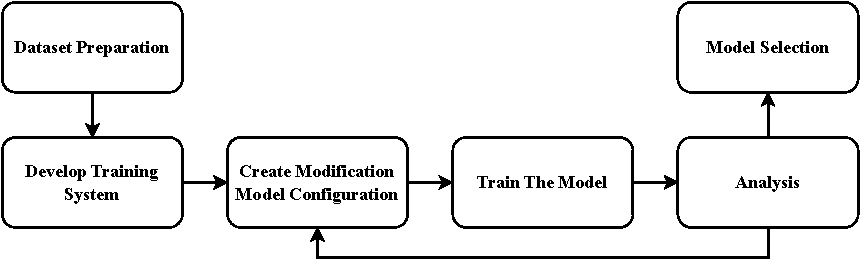
\includegraphics[width=.9\textwidth]{figures/methods.pdf}
  \caption{Search Steps}
  \label{fig:methods}
\end{figure}
\vspace{-1ex}
  %insert diagram modifikasi here
  %Menyiapkan dataset, Membuat \emph{auto-trainer}, Membuat konfigurasi-konfigurasi modifikasi, Melatih model-model YOLOv7 yang sudah dimodifikasi,
  %Menganalisis performa hasil modifikasi YOLOv7, dan Pemilihan model modifikasi YOLOv7 dengan skor mAP terbaik.

  %Pada tahap persiapan dataset, akan dilakukan pengunduhan dataset dari \textcite{aot_dataset}.
  %Gambar-gambar pada dataset ini kemudian akan di-\emph{sampling} dan didistribusikan menjadi dataset \emph{training}, validasi, dan pengujian.
  %Pada pendistribusian dataset ini juga akan dilakukan \emph{balancing} antar kelas dan dataset positif negatif.
  %\emph{Balancing} dilakukan agar tidak ada kelas yang mendominasi pada dataset.

  %Selanjutnya, di tahap pembuatan \emph{auto-trainer}, akan dilakukan pembuatan program yang dapat dengan otomatis membangun dan melatih \emph{neural network} modifikasi YOLOv7.
  %Pembuatan \emph{auto-trainer} ini dilakukan agar proses-proses pengerjaan tahapan-tahapan selanjutnya menjadi dapat dilakukan dengan lebih mudah.

  %Setelah itu, akan dilakukan pembuatan konfigurasi-konfigurasi modifikasi.
  %Konfigurasi modifikasi YOLOv7 akan dibuat agar dapat diinputkan pada \emph{auto-trainer}.
  %Konfigurasi modifikasi akan berisi kombinasi modifikasi-modifikasi yang ada pada subbab \ref{section:modificationcandidates}.

  %Tahapan selanjutnya adalah \emph{Training} model.
  %Pada tahap ini, konfigurasi-konfigurasi modifikasi pada tahapan sebelumnya akan dibangun dan kemudian dilatih.
  %Model akan dilatih \emph{from scratch}. Dengan kata lain, model tidak akan dilatih dengan menggunakan \emph{pre-trained weights}.
  %Hasil dari tahap ini adalah \emph{weights neural network} modifikasi YOLOv7, histori pelatihannya, dan metrik-metriknya pada dataset uji.

  %Pada tahap analisis, hasil dari tahap sebelumnya akan dianalisis untuk mencari tahu performa model-model hasil modifikasi.
  %Analisis juga dilakukan untuk menemukan \emph{gap} kandidat modifikasi lain yang masih bisa dieksplorasi untuk meningkatkan kemampuan pendeteksian objek kecil YOLOv7.
  %Ketika suatu kandidat modifikasi seperti itu ditemukan, maka akan dilakukan kembali pembuatan konfigurasi modifikasi untuk menguji kandidat modifikasi baru tersebut.

To conduct this research, we first have to prepare the dataset.
First, the dataset will be downloaded from \textcite{aot_dataset}.
Then, the labels of the dataset will be converted to darknet or COCO format.
Next, the dataset will be sampled into training set, validation set, and test set.
The sampling will be done in a way that balances the number classes in each set so
that there will be no dominating class during training.
  
The next thing to do is to develop a training system.
The purpose of this system is to make the training process easily conducted and monitored.
This system will include features such as train fail notification, train queueing, and alert the user
when the computer overheats.

Moving on, we have model configuration creation. Here we will create a model configuration file based on the 
modification that we want to try. The modification configurations will be made according to the modification
candidates listed in section \ref{section:modificationcandidates}.

The next step is to train the model.
The model configurations that was made in previous step will be built and trained from scratch (no pre-trained weights).
In this step, the weights of the neural network, training history, and performance metrics will be generated for analysis.

In the analysis step, we will analyze the performance of the modified YOLOv7.
This step is done to find other candidate of modification that might work.
If such modification candidate was found, we will go back to create the model configuration, 
and then train the modification.

Finally, in the last step we will select the best model.
We will select the model with the best performance among the modified YOLOv7 models.
The model selection will be done based on $mAP@50$ metric, with constraint in inference latency.
The model that qualify for selection must be able to perform inference with speed of atleast 10 FPS in a consumer GPU Nvidia RTX 2080Ti.
  %Tahapan terakhir adalah pemilihan model terbaik.
  %Pada tahapan ini akan dipilih model yang memiliki performa terbaik dari antara model-model hasil modifikasi lainnya.
  %Pemilihan model akan dilakukan dengan berdasarkan pada skor mAP tertinggi.
  %Untuk mempertahankan solusi optimisasi yang dapat melakukan deteksi secara \emph{real time}, model yang akan dipilih adalah model yang dapat melakukan deteksi yang cukup cepat pada \emph{edge} GPU.


\section{Modification Candidates}
\label{section:modificationcandidates}
  \subsection{Mosaic Augmentation}
  As discussed in section \ref{section:mosaic_study}, mosaic augmentation was able to increase the detection accuracy of small objects
  on many object detection neural networks. For this reason, we will experiment by training YOLOv7 with and without  mosaic augmentation.
    %Seperti yang dibahas pada subbab \ref{section:mosaic_study}, augmentasi mosaic pada dataset mampu meningkatkan akurasi deteksi objek-objek kecil dari model.
    %Oleh karena itu, akan dilakukan eksperimen menambahkan augmentasi mosaik pada YOLOv7 untuk melihat apakah augmentasi ini akan meningkatkan akurasi, khususnya pada dataset objek kecil.
  \subsection{Pre-training Anchor Recalculation}
    %Yang dimaksud dengan rekalkulasi \emph{anchor on-training}  adalah ketika ukuran-ukuran \emph{anchor box} direkalkulasi pada saat training.
    %Berbeda dengan \emph{clustering pre-training} seperti pada YOLOv2 \parencite{yolov2}, ukuran-ukuran \emph{anchor} akan di-\emph{learning} bersama dengan pendeteksi objeknya.
    %Untuk melakukan hal ini, digunakan algoritma optimisasi \emph{anchor box} yang mirip dengan algoritma \textcite{anchoropt}.
    %Pada bagian \emph{head}, akan ditempelkan suatu layer yang akan mengoutputkan faktor \emph{rescaling} dari tiap \emph{anchor box}.
    %Bagian tersebut akan di-\emph{training} bersama dengan YOLOv7 \emph{anchor box} akan teroptimisasi tidak hanya pada dataset, namun pada keseluruhan \emph{neural network} juga.

    %Anchor yang disediakan pada kode implementasi dari YOLOv7 merupakan anchor yang dikalkulasi untuk mengoptimisasi deteksi pada dataset
    %COCO2017. Dengan pertimbangan bahwa distribusi dataset yang akan digunakan pada penelitian ini berbeda dari objek general di COCO2017,
    %maka anchor harus direkalkulasi. Dengan melakukan rekalkulasi anchor, tiap layer head pada YOLOv7 akan dengan lebih mudah mem-\emph{fit}
    %objek-objek yang ada pada gambar.
  In the implementation code of YOLOv7, the anchors provided was calculated based on COCO2017 dataset.
  We assume that the dataset distribution of airborne objects to be greatly different from COCO2017.
  As such, the anchors must be recalculated for faster learning. This recalculation will be conducted
  using k-means algorithm. One problem however is that k-means might fail to cluster the dataset into 
  the amount of anchors that we needed. To tackle this, we might have to cluster it in logarithmic coordinates. 

  \subsection{Replacing Localization Loss to Extended IoU}
  \begin{figure}[H]
      \centering
      \begin{subfigure}[][][t]{0.3\textwidth}
        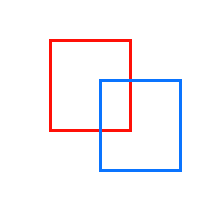
\includegraphics[width=1\linewidth]{figures/iounot0.png}
        \caption{$IoU > 0$ when 2 boxes intersect}
        \label{fig:iouexist}
      \end{subfigure}\hfill
      \begin{subfigure}[][][t]{0.3\textwidth}
        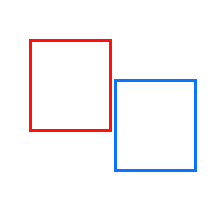
\includegraphics[width=1\linewidth]{figures/iou0near.png}
        \caption{$IoU = 0$ when 2 boxes does not intersect}
        \label{fig:iou0near}
      \end{subfigure}\hfill
      \begin{subfigure}[][][t]{0.3\textwidth}
        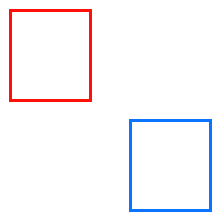
\includegraphics[width=1\linewidth]{figures/iou0far.png}
        \caption{$IoU = 0$ when 2 boxes does not intersect and far away}
        \label{fig:iou0far}
      \end{subfigure}
      \caption{Cause of IoU vanishing gradient}
      \label{fig:iouvanishinggrad}
  \end{figure}
  Extended-IoU (EIoU) is a modification of IoU that are used in neural networks to tackle
  the problem of vanishing gradient \parencite{eiou}. 
  IoU are known to cause vanishing gradient problem due to its behavior when two bounding boxes are not intersecting.
  When 2 boxes $A$ and $B$ are not intersecting, the area of intersection ($A\cap B$) would always be 0.
  This value doesn't give any information whether the boxes are far apart (Figure \ref{fig:iou0far}) or 
  near but not intersecting (Figure \ref{fig:iou0near}).
  To solve this, loss involving $IoU$ are usually paired with some regularization terms.
  For example \textcites{giou}{diou_ciou} proposed $GIoU$, $DIoU$, and $CIoU$.
  
  YOLOv7 itself is using $CIoU$ for its localization loss. $CIoU$ is just regular $IoU$
  that is paired with distance and box aspect ratio regularization terms.
  The problem of these kinds of regularized IoU is that when the boxes intersect, it does not
  behave like IoU anymore. $GIoU$, $DIoU$ and $CIoU$ have residue of their regularization when
  the boxes intersect. Metrics used to evaluate object detection
  algorithms depend on IoU (\textit{e.g.\ mAP}).
  For this reason \textcite{eiou} designed EIoU. The main appeal of EIoU
  is that it behave exactly like IoU when the boxes intersect and gives non-positive value when the
  boxes do not intersect.
  By behaving exactly like IoU, it is hoped that the model would perform better on the metrics.


    %\emph{Extended} IoU (EIoU) merupakan salahsatu modifikasi dari
    %IoU yang dibuat untuk menyelesaikan permasalahan \emph{vanishing gradient}
    %pada IoU \parencite{eiou}. Hal yang menyebabkan IoU bermasalah dengan \emph{vanishing gradient}
    %adalah nilai dari IoU yang selalu menjadi 0 ketika 2 \emph{bounding box} tidak beririsan.
    %Permasalahan ini diselesaikan oleh EIoU dengan memberikan nilai negatif untuk 
    %bounding box yang tidak beririsan, sehingga neural network dapat mengoptimasi loss function $-EIoU$.
    %Teknik konveksikasi juga dapat dilakukan dengan mengoptimasi $(1-EIoU)^2$

    %YOLOv7 sendiri menggunakan CIoU sebagai localization loss. CIoU juga merupakan suatu solusi
    %dari permasalahan \emph{vanishing gradient}. CIoU menambahkan suku jarak antar bounding box 
    %dan kecocokan \emph{aspect ratio} antar boundingbox pada IoU. Keunggulan EIoU daripada CIoU
    %adalah EIoU akan bertingkah seperti IoU ketika bounding box beririsan. Karena metrik-metrik
    %yang digunakan untuk mengukur kemampuan deteksi dilakukan berdasarkan IoU, dianggap akan
    %lebih baik jika loss yang digunakan sama seperti metriknya \parencite{eiou}.

  \subsection{Utilizing Earlier Feature Map Stage}
    %\begin{figure}[ht]
    %  \centering
    %  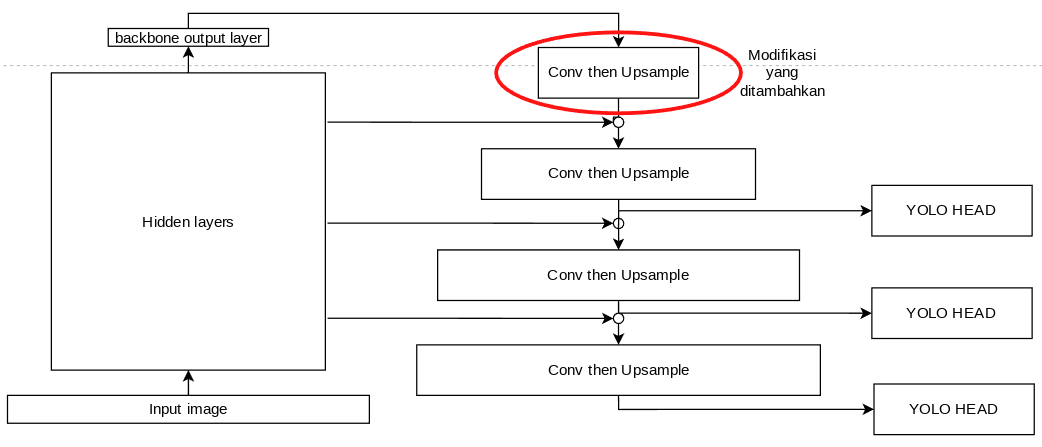
\includegraphics[scale=0.5]{figures/add-more-upsampling.png}
    %  \caption{Menambah \emph{upsampling} pada \emph{neck}}
    %  \label{fig:neckaddupsampling}
    %\end{figure}

  \begin{figure}[H]
    \centering
    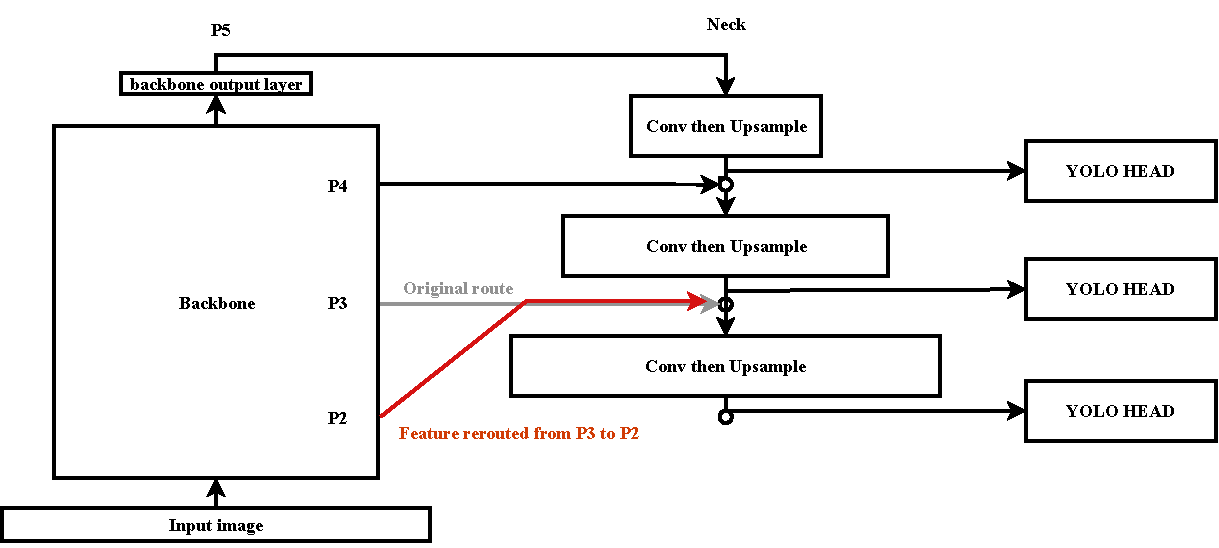
\includegraphics[width=.9\textwidth]{figures/neck-move-back.pdf}
    \caption{Rerouting Neck Connection to Earlier Stage}
    \label{fig:neckmoveback}
  \end{figure}
  In a deep neural network, the extracted feature/abstraction of the data become more prominent
  as the input data passes through deeper layers. However, information loss also increases in the
  deeper layer. For small object detection, information is crucial. There is a posibility the features
  of small objects are lost as the data propagates through the network.
  
  If we view it in a data path network design perspective, the greater the length of the path from input
  to output, the more information will be lost. Therefore, we propose to reroute the orignal connection from
  backbone to the neck to an earlier stage of inference. For example, YOLOv7 take feature maps from P3, P4, and P5
  scales of the backbone, we can reroute the connection from P3 to P2 as shown in Figure \ref{fig:neckmoveback}.
  %Seperti pada penelitian-penelitian terkait di subbab \ref{section:relatedwork}, modifikasi \emph{neck} dapat dilakukan untuk meningkatkan akurasi pendeteksian objek kecil.
  %Modifikasi koneksi \emph{neck} ke \emph{backbone} dapat dilakukan dengan memindahkan sumber feature map untuk beberapa layer neck lebih jauh ke belakang seperti pada Gambar \ref{fig:neckmoveback}.
  %%Penambahan layer upsampling dapat membuat neural network untuk mendapatkan feature-map yang lebih detail sehingga dapat melakukan pendeteksian objek kecil dengan lebih baik.
  %Pemindahan sumber feature map ke belakang dapat dilakukan untuk mengantisipasi fitur objek kecil yang bisa saja hilang ketika layer neural network semakin dalam.
  %Dengan memindahkannya lebih ke belakang, YOLOv7 akan melakukan deteksi dengan memanfaatkan fitur yang abstraksi yang lebih rendah tetapi sedikit informasi yang hilang.
  \subsection{Additional YOLO Head}
  \begin{figure}[H]
    \centering
    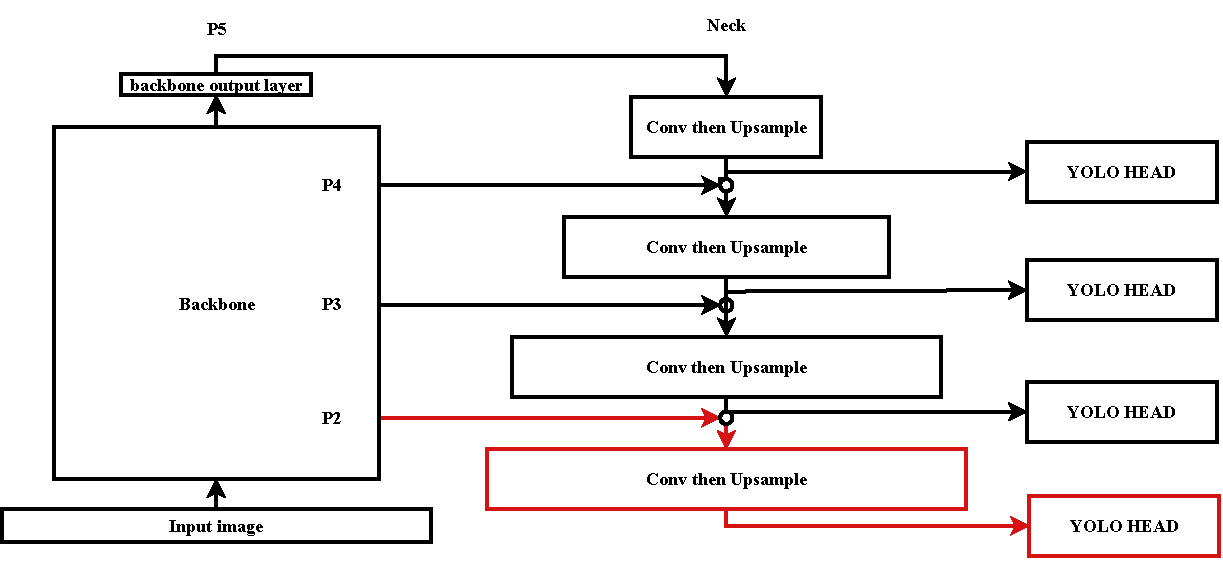
\includegraphics[width=.9\textwidth]{figures/addmorehead.pdf}
    \caption{Adding an Extra Head Layer}
    \label{fig:addmorehead}
  \end{figure}
  An additional YOLO head means an extra stage of detection.
  With more stage of detection, the large variance of the objects in the dataset can be learned.
  This is especially good for \textcite{aot_dataset} where the area of the bounding boxes in the dataset
  can be orders of magnitude apart (see section \ref{section:dataset}).
  
  %%Penambahan YOLO head dapat membuat YOLOv7 melakukan deteksi pada skala yang lebih banyak.
  %%Hal ini akan berpengaruh pada kemampuan pendeteksian objek kecil.
  %%Dengan melakukan pendeteksian pada skala yang lebih banyak, YOLOv7 dapat mendeteksi objek yang besar maupun kecil.
  %Perhatikan bahwa penambahan YOLO Head akan diikuti dengan penambahan \emph{layer upsampling} pada \emph{neck} seperti di Gambar \ref{fig:addmorehead}.

  \subsection{Replace YOLO Head to YOLOX's Decoupled Anchor-free Head}
  \begin{figure}[H]
    \centering
    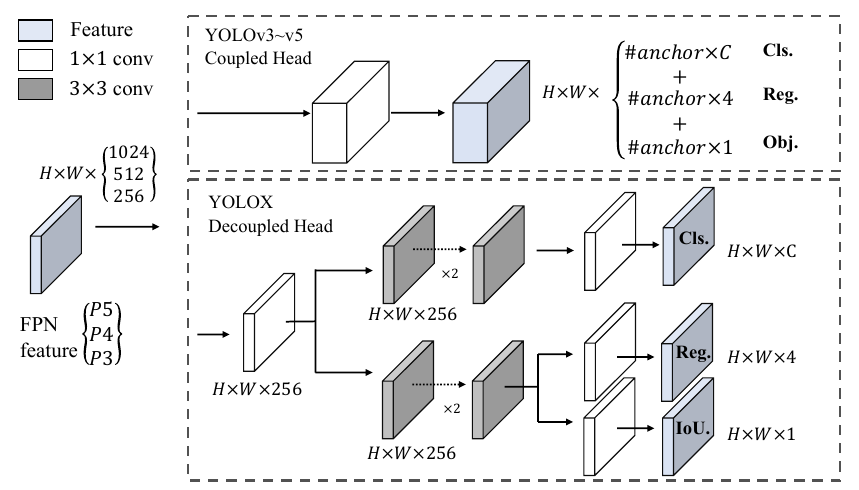
\includegraphics[width=0.8\textwidth]{figures/anchorfree-yolox.png}
    \caption{Decoupled Anchor-free Head in YOLOX compared to Coupled Head in mainstream YOLO}
    \label{fig:anchorfree}
  \end{figure}

  YOLOv6 and YOLOX used a different kind of head layer compared to usual YOLO \parencites{yolox}{yolov6}. 
  In mainstream YOLO, prediction for bounding box and classes are both calculated on the same layer.
  With decoupled anchor-free head, the layers are separated for class prediction and bounding box prediction, and
  bounding box prediction are done using 4 value without anchor as seen on Figure \ref{fig:anchorfree}. 
  Using decoupled anchor-free head gives us 2 advantages. 1) Reducing the amount of design parameters as 
  we don't have to introduce anchor boxes to the model. 2) Reducing the complexity of interpreting prediction
  result. Advantage (1) is especially enticing. There is a possibility of us introducing bad priors to the neural
  network by poorly clustering anchor boxes. By having a model that less dependent on prior, we can reduce such possibility.

  A thing to consider when applying decoupled anchor-free head to YOLOv7 is the label assigner. YOLOv7 and YOLOX uses SimOTA as its default
  label assigner. However, \textcite{yolov6} YOLOv6 uses Task-aligned Assigner (TAL) for its label assigner. They reported that TAL performs
  better than SimOTA. Therefore, in applying decoupled anchor-free head, it might be better to use TAL as label assigner.
  %Decoupled head gives us 2 advantages. 
  %1) Reducing the amount of


  %Pada YOLOX, \emph{coupled anchor head} seperti pada arsitektur YOLO pada umumnya diganti dengan \emph{decoupled anchor-free head} \parencite{yolox}.
  %Keuntungan dari model anchor-free adalah kita tidak perlu mendefinisikan \emph{anchor} sebelum melakukan training sehingga mengurangi beberapa proses
  %tuning heuristik seperti rekalkulasi anchor. Memakai \emph{head} yang anchor free juga memberi kompleksitas proses training dan pendekodean output model.
  %\cite{yolox} melaporkan peningkatan pada akurasi dan pengurangan parameter sehingga mempercepat lama deteksi.
  %Oleh karena hal-hal tersebut, mencoba memakai \emph{head anchor-free} di YOLOv7 baik untuk dicoba.
    
    
\section{Dataset}
\label{section:dataset}

  \subsection{Source}
  \label{section:datasetsource}
  Dataset containing annotated images of airborne objects can be obtained from \textcite{aot_dataset}.
  This dataset is hosted in an AWS S3 Bucket.
  The dataset consist of several Unmanned Aerial Vehicle (UAV) flights' frame-by-frame camera capture.
  There are 7 classes in the dataset but most there are 3 dominating classes.
  The size of the dataset and its class distribution can be seen on Figure \ref{tbl:datasettraintest} and
  \ref{tbl:datasetclasses} respectively.
  %Dataset untuk objek-objek \emph{airborne} didapatkan dari \textcite{aot_dataset} dan dihost pada suatu server AWS S3 Bucket.
  %Dataset ini berisi video-video monokromatik penerbangan UAV.
  %Terdapat 4 kelas pada dataset ini yaitu pesawat, helikopter, burung, dan \emph{other}.
  %Distribusi dataset training dan uji dapat dilihat pada tabel \ref{tbl:datasettraintest} sedangkan distribusi kelas dari dataset dapat dilihat pada Tabel \ref{tbl:datasetclasses}.
  \begin{table}[H]
    \centering
    \captionof{table}{Original Dataset Splits}
    \label{tbl:datasettraintest}
    
\begin{table}[H]
  \centering
  \captionof{table}{Distribusi Dataset Training dan Test}
  \label{tbl:datasettraintest}
  \begin{tabular}{|c|c|c|c|c|}
    \hline
    Pembagian & Ukuran (TB) & Sekuen penerbangan & Jumlah Gambar & Jumlah Label\\
    Dataset &  & UAV &  & \\
    \hline
    Training & 11,3 & 4154 & 4975765 & 2891891\\
    \hline
    Validation + Test &2.1 &789 & 943852 & 496075\\
    \hline
    Total &13,4 &4943 & 5919617 & 3387966\\
    \hline
  \end{tabular}
\end{table}
  \end{table}
  \begin{table}[H]
    \centering
    \captionof{table}{Dataset' Objects Classes Distribution}
    \label{tbl:datasetclasses}
    \begin{tabular}{ c c c c c c }
  \toprule[1.5pt]
  Splits & Total Objects & Airplane & Helicopter & Bird & \emph{Other 4 Classes}\\
  \midrule
  Training & 2,89 M & 0,79 M& 1,22 M& 0,33 M& 0,54 M\\
  Validation + Test &0,50 M &0,13 M & 0,17 M&0,06 M&0,14 M\\
  \midrule
  Total &3,39 M &0,92 M & 1,39 M&0,39 M&0,69 M\\
  \bottomrule[1.5pt]
\end{tabular}
  \end{table}
  %Kebanyakan \emph{bounding box} pada dataset berukuran sangat kecil.
  %Distribusi dari luas \emph{boudning box} dapat dilihat pada gambar \ref{fig:areadist}.
  %Perhatikan pada gambar tersebut, sumbu x menggunakan skala logaritmik.
  %Sebagai referensi, luas dari tiap frame itu sekitar $5\times10^16 px^2$.
  %\begin{figure}[H]
  %  \centering
  %  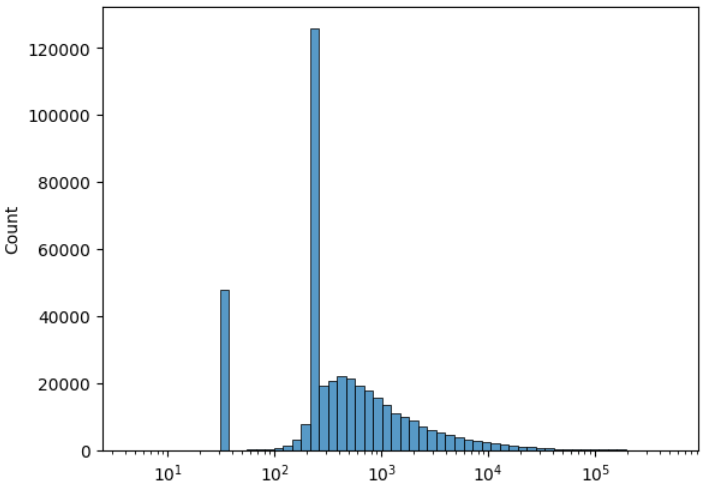
\includegraphics[scale=0.65]{figures/area-dist.png}
  %  \caption{Penambahan \emph{Layer} Head pada YOLO}
  %  \label{fig:areadist}
  %\end{figure}

  
  \subsection{Sampling Dataset}
  As seen on section \ref{section:datasetsource}, The size of the dataset is massive.
  Due to the limitation of computational resource, we will only able to sample some of them
  for training and testing. We will sample in total 700 images from the dataset with splits
  as shown in Table \ref{tbl:datasetsamplingdist}.
  %Karena jumlah dataset pada \textcite{aot_dataset} berukuran sangat besar, dan keterbatasan
  %\emph{computational resource}, hanya sebagian dari dataset tersebut akan digunakan untuk \emph{training} dan \emph{test}.
  %Akan diambil total 700 gambar dari dataset dengan pembagian sesuai dengan Tabel \ref{tbl:datasetsamplingdist}
  \begin{table}[H]
    \centering
    \captionof{table}{Distribusi Sampling Dataset}
    \label{tbl:datasetsamplingdist}
    \begin{tabular}{c c c c c c c}
      \toprule[1.5pt]
      Splits    &Total &\multicolumn{5}{c}{Classes Percentage}\\
                        \cline{3-7}
                &Images& Airplane & Helicopter & Bird & Drone & Negative\\
      \midrule
      Training  &400   &23.75\%   &23.75\%     &23.75\% &23.75\%       &5\%\\
      \midrule
      Validation&100   &20\%      &20\%        &20\%    &20\%          &20\%\\
      \midrule
      Test      &200   &20\%      &20\%        &20\%    &20\%          &20\%\\
      \bottomrule[1.5pt]
    \end{tabular}
  \end{table}

  %Untuk membagi dataset agar terdistribusi seperti pada Tabel \ref{tbl:datasetsamplingdist}, akan digunakan algoritma seperti berikut:
  %\begin{algorithmic}
  %  \State $L_0 \gets$ List index gambar-gambar yang memiliki objek kelas pesawat
  %  \State $L_1 \gets$ List index gambar-gambar yang memiliki objek kelas helikopter
  %  \State $L_2 \gets$ List index gambar-gambar yang memiliki objek kelas burung 
  %  \State $L_3 \gets$ List index gambar-gambar yang memiliki objek kelas \emph{Other}
  %  \State $L_4 \gets$ List index gambar-gambar yang memiliki objek kelas negatif
  %  \For{$i \gets 0$ to $4$}
  %    \State $L_i \gets shuffle(L_i)$
  %  
  %  

  %\end{algorithmic}

\section{Instruments}
To conduct this research, we will be using a computer with the following specs:
\begin{itemize}[noitemsep,topsep=0pt,leftmargin=.1\textwidth,rightmargin=.1\textwidth]
  \item CPU \hfill Intel® Core™ i5-9400F CPU @ 2.90GHz
  \item GPU \hfill Nvidia Geforce RTX 2080 Ti
  \begin{itemize}[noitemsep,topsep=0pt]
    \item[] Memory \hfill 11 GB
    \item[] CUDA Compute Capability \hfill 7.5
  \end{itemize}
  \item RAM \hfill 12 GB
  \item Hard Drive Available Memory \hfill 1.3 TB
  \item Operating System \hfill Ubuntu 20.04
  \item Cuda Toolkit Version \hfill 11.7
  \item PyTorch Version \hfill 1.13.1
\end{itemize}
%\begin{tabular}{>{\hspace{1em}}l >{\hspace{1pt}}l >{\hspace{3em}}l}
  CPU &       & Intel® Core™ i5-9400F CPU @ 2.90GHz\\
  GPU &       & Nvidia Geforce RTX 2080 Ti\\
      &Memory & 12 GB\\
      &Cuda CC& 7.5\\
  RAM &       & 12 GB\\

\end{tabular}

%\begin{itemize}[noitemsep,topsep=0pt]
%  \item CPU \hfill Intel(R) Core(TM) i5-9400F CPU @ 2.90GHz
%  \item GPU \hfill Nvidia Geforce RTX 2080 Ti
%  \begin{itemize}[noitemsep,topsep=0pt]
%    \item[] Memory \hfill 12 GB
%    \item[] CUDA Compute Capability \hfill 7.5
%  \end{itemize}
%  \item RAM \hfill 12 GB
%  \item Disk Available Memory \hfill 1.3 TB
%  \item Operating System \hfill Ubuntu 20.04
%  \item Cuda Toolkit Version \hfill 11.7
%  \item PyTorch Version \hfill 1.13.1
%\
  %Untuk melaksanakan eksperimen ini, akan digunakan suatu komputer yang dilengkapi dengan
  %GPU Nvidia RTX 2080 Ti yang memiliki kapasitas 11GB VRAM. Oleh karena keterbatasan ini,
  %Melatih model-model YOLOv7 besar seperti W6, E6, dan E2E yang dimodifikasi menjadi sangat sulit,
  %apalagi pada skala input sesuai dengan dimensi dataset.
  %Oleh karena hal ini, arsitektur yang akan dipilih sebagai \emph{baseline} modifikasi adalah YOLOv7 dengan
  %ukuran normal karena model tersebut adalah model terbesar yang mampu di-\emph{train} pada RTX 2080 Ti dengan 
  %input size 1600x1600 dan batch size 1.

  %Selain itu, jumlah dataset yang akan digunakan juga akan dibatasi menjadi 400 seperti pada subbab \ref{section:dataset} untuk menghemat waktu training.
  %Pada pilot test, ditemukan bahwa dibutuhkan sekitar 20 jam untuk men-\emph{train} model sebanyak 300 epoch pada dataset dengan 400 gambar jika menggunakan
  %GPU RTX 2080 Ti.





%\section{Skema Training Model}
%  Untuk melatih berbagai modifikasi YOLOv7, akan dibuat suatu \emph{auto-trainer}.
%  \emph{Auto-trainer} ini akan menerima suatu \emph{file} konfigurasi modifikasi YOLOv7, dan dengan otomatis membangun arsitektur YOLOv7 yang termodifikasi dan melatihnya.
%  Setelah mendapatkan model modifikasi YOLOv7 yang sudah dilatih, \emph{auto-trainer} akan menguji model tersebut dengan dataset uji.
%  Metrik-metrik pengujian, grafik histori \emph{training loss vs validation loss}, dan \emph{weights} dari model kemudian akan dikirim ke user.
%  Dengan membuat \emph{auto-trainer} ini, proses pelatihan model dan pelaporan hasil menjadi terotomasi sehingga akan mempermudah proses penelitian.
%
%\section{Timeline Pelaksanaan Penelitian}
%  \newcommand{\w}{}
%  \newcommand{\G}{\cellcolor{gray}}
%  \begin{table}[h!]
%    \captionof{table}{Tabel timeline}
%    \label{tbl:timeline}
%    \begin{tabular}{|p{3.5cm}|c|c|c|c|c|c|c|c|c|c|c|c|c|c|c|c|}
%  
%      \hline
%      \multirow{2}{*}{Kegiatan} & \multicolumn{16}{|c|}{Minggu} \\
%      \cline{2-17} &
%      1 & 2 & 3 & 4 & 5 & 6 & 7 & 8 & 9 & 10 & 11 & 12 & 13 & 14 & 15 & 16 \\
%      \hline
%  
%      % Gunakan \G untuk mengisi sel dan \w untuk mengosongkan sel
%      Persiapan Dataset &
%      \G & \w & \w & \w & \w & \w & \w & \w & \w & \w & \w & \w & \w & \w & \w & \w \\
%      \hline
%  
%      Pemb. \emph{Auto-trainer} &
%      \w & \G & \w & \w & \w & \w & \w & \w & \w & \w & \w & \w & \w & \w & \w & \w \\
%      \hline
%  
%      Pemb. Konfigurasi&
%      \w & \w & \G & \G & \G & \G & \G & \G & \G & \G & \G & \G & \w & \w & \w & \w \\
%      Modifikasi &
%      \w & \w & \G & \G & \G & \G & \G & \G & \G & \G & \G & \G & \w & \w & \w & \w \\
%      \hline
%  
%      Training Model &
%      \w & \w & \G & \G & \G & \G & \G & \G & \G & \G & \G & \G & \w & \w & \w & \w \\
%      \hline
%
%      Analisis &
%      \w & \w & \G & \G & \G & \G & \G & \G & \G & \G & \G & \G & \G & \w & \w & \w \\
%      \hline
%
%      Pemb. Laporan &
%      \w & \w & \w & \w & \w & \w & \w & \w & \w & \w & \w & \w & \G & \G & \G & \G \\
%      \hline
%  
%    \end{tabular}
%  \end{table}

  \newpage

  % Konten lainnya
  % \input{contents/4-lainnya.tex}

  % Daftar pustaka
  \chapter*{DAFTAR PUSTAKA}
  \addcontentsline{toc}{chapter}{DAFTAR PUSTAKA}
  \renewcommand\refname{}
  \vspace{2ex}
  \renewcommand{\bibname}{}
  \begingroup
    \def\chapter*#1{}
    \printbibliography
  \endgroup
  \chapter{dummy}
  \chapter{dummy}
  \chapter{dummy}
  \chapter{dummy}
  \chapter{dummy}
  \chapter{dummy}
  \chapter{dummy}
  \chapter{dummy}
  \chapter{dummy}
  \chapter{dummy}


\end{document}
